\documentclass[a4paper,11pt,reqno]{amsart}
\renewcommand{\baselinestretch}{1.1}

\usepackage{amsmath}
\usepackage{amsfonts}
\usepackage{amssymb}
\usepackage{amsthm}
\usepackage[shortlabels]{enumitem}
\usepackage{graphicx}
\usepackage{color}
\usepackage{dsfont}
\usepackage[latin1]{inputenc}
\usepackage{MnSymbol}
\usepackage{enumitem}
\usepackage{extpfeil}
\usepackage{mathtools}
\usepackage{url}
\usepackage[margin=1in]{geometry}
\usepackage{fancyhdr}
\usepackage[all,cmtip]{xy}


\fancyhf{}
\fancyhead[C]{\thepage}
\pagestyle{fancy}
\headheight = 13pt


\numberwithin{equation}{section}


\title{K\"ahler groups and subdirect products of surface groups}
\author{Claudio Llosa Isenrich}
\address{Laboratoire de Math\'ematiques d'Orsay, Univ. Paris-Sud, CNRS, Universit\'e Paris-Saclay, 91405 Orsay, France}

\email{claudio.llosa-isenrich@math.u-psud.fr}
\thanks{This work was supported by a EPSRC Research Studentship, by the German National Academic Foundation, and by a public grant as part of the FMJH}
\keywords{K\"ahler groups, Branched covers, Homological finiteness properties}
\subjclass[2010]{32J27 (32Q15, 20F65, 20J05)}



\begin{document}

%%Confirmation Thesis Version


\newcommand{\AAA}{{\mathds A}}
\newcommand{\CC}{{\mathds C}}
\newcommand{\PP}{{\mathbf P}}
\newcommand{\QQ}{{\mathds Q}}
\newcommand{\RR}{{\mathds R}}
\newcommand{\NN}{{\mathds N}}
\newcommand{\ZZ}{{\mathds Z}}
\newcommand{\del}{{\partial}}
\newcommand{\one}{{\mathds {1}}}
\newcommand{\ord}{{\mathcal {O}}}
\newcommand{\ii}{{\mathds {i}}}
\newcommand{\vol}{{\mathrm {vol}}}
\newcommand{\eps}{{\epsilon}}
\def\Mod{{\rm{Mod}}}
\def\C{{\mathds C}}
\def\D{{\rm D}}
\def\S{\Sigma}
\def\F{{\mathds F}}
\def\FF{\mathcal F}
\def\aut{{\rm{Aut}}}
\def\inn{{\rm{Inn}}}
\def\out{{\rm{Out}}}
\def\isom{{\rm{Isom}}}
\def\mcg{{\rm{MCG}}}
\def\ker{{\rm{ker}}}
\def\im{{\rm{im}}}
\def\dim{{\rm{dim}}}
\def\G{\Gamma}
\def\a{\alpha}
\def\g{\gamma}
\def\L{\Lambda}
\def\Z{{\mathds{Z}}}
\def\H{{\mathds{H}}}
\def\n{{\bf N}}
\newcommand{\mm}{{\underline{m}}}
\newcommand{\nn}{{\underline{n}}}




\theoremstyle{plain}
\newtheorem{theorem}{Theorem}[section]
\newtheorem{acknowledgement}[theorem]{Acknowledgement}
\newtheorem{claim}[theorem]{Claim}
\newtheorem{conjecture}[theorem]{Conjecture}
\newtheorem{corollary}[theorem]{Corollary}
\newtheorem{exercise}[theorem]{Exercise}
\newtheorem{lemma}[theorem]{Lemma}
\newtheorem{proposition}[theorem]{Proposition}
\newtheorem{question}{Question}
\newtheorem*{thmIntro1}{Theorem \ref{thmNewCoab}}
\newtheorem*{question2}{Question \ref{qnIntroKGsFinProps}}
\newtheorem*{question3}{Question \ref{qnIntroSuciuFinPres}}
\newtheorem*{question*}{Question}
\newtheorem{addendum}[theorem]{Addendum}

\newtheorem{keytheorem}{Theorem}
\renewcommand{\thekeytheorem}{\Alph{keytheorem}}



\theoremstyle{definition}
\newtheorem{remark}[theorem]{Remark}
\newtheorem*{acknowledgements*}{Acknowledgements}
\newtheorem{example}[theorem]{Example}
\newtheorem{definition}[theorem]{Definition}
\newtheorem*{notation*}{Notation}
\newtheorem*{convention*}{Convention}

%
\renewcommand{\proofname}{Proof}


%%%%%%%%%%%%%%%%%%%%%%%%%%%%%%%%%%%%%%%%%%%%%%%%%%%%%%%%%%%%%%
%%% OWN THEOREM-LIKE ENVIRONMENTS
%%%%%%%%%%%%%%%%%%%%%%%%%%%%%%%%%%%%%%%%%%%%%%%%%%%%%%%%%%%%%%
%\theoremstyle{plain}
%\newtheorem{theorem}{Theorem}[section]
%\newtheorem{acknowledgement}[theorem]{Acknowledgement}
%\newtheorem{algorithm}[theorem]{Algorithm}
%\newtheorem{axiom}[theorem]{Axiom}
%\newtheorem{case}[theorem]{Case}
%\newtheorem{claim}[theorem]{Claim}
%\newtheorem{conclusion}[theorem]{Conclusion}
%\newtheorem{condition}[theorem]{Condition}
%\newtheorem{conjecture}[theorem]{Conjecture}
%\newtheorem{korollar}[theorem]{Korollar}
%\newtheorem{corollary}[theorem]{Corollary}
%\newtheorem{criterion}[theorem]{Criterion}
%\newtheorem{exercise}[theorem]{Exercise}
%\newtheorem{lemma}[theorem]{Lemma}
%\newtheorem{notation}[theorem]{Notation}
%\newtheorem{problem}[theorem]{Problem}
%\newtheorem{proposition}[theorem]{Proposition}
%\newtheorem{question}{Question}
%\newtheorem{solution}[theorem]{Solution}
%\newtheorem{summary}[theorem]{Summary}
%
%\newtheorem{satz}[theorem]{Satz}
%
%\theoremstyle{definition}
%\newtheorem{definition}[theorem]{Definition}
%\newtheorem{bemerkung}[theorem]{Bemerkung}
%\newtheorem{beispiel}[theorem]{Beispiel}
%\newtheorem{remark}[theorem]{Remark}
%\newtheorem*{acknowledgements*}{Acknowledgements}
%\newtheorem{example}[theorem]{Example}
%
%%
%\renewcommand{\proofname}{Proof}

 
\begin{abstract}
We present a construction that produces infinite classes of K\"ahler groups that arise as fundamental groups of fibres of maps to higher dimensional tori. Following the work of Delzant and Gromov, there is great interest in knowing which subgroups of direct products of surface groups are K\"ahler.  We apply our construction to obtain new classes of irreducible, coabelian K\"ahler subgroups of direct products of $r$ surface groups. These cover the full range of possible finiteness properties of irreducible subgroups of direct products of surface groups: For any $r\geq 3$ and $2\leq k \leq r-1$, our classes of subgroups contain K\"ahler groups that have a classifying space with finite $k$-skeleton while not having a classifying space with finitely many $(k+1)$-cells. 

We also address the converse question of finding constraints on K\"ahler subdirect products of surface groups and, more generally, on homomorphisms from K\"ahler groups to direct products of surface groups. We show that if a K\"ahler subdirect product of $r$ surface groups admits a classifying space with finite $k$-skeleton for $k>\frac{r}{2}$, then it is virtually the kernel of an epimorphism from a direct product of surface groups onto a free abelian group of even rank.
\end{abstract}

\maketitle



\section{Introduction}
The presence of sensors in the ubiquitous environment has led to the production of an enormous amount of data. These sensors belong to diverse categories including planar pressure, thermal, optical, acoustic, and proximity modalities. 
They provide information for activity recognition and context-aware models that could be used for a wide range of applications such as automatic monitoring in the smart environment and wellness scene, computer-human-interaction, user experience, etc. 
%The information and feedback provided by the sensors are used to get the context in which they are placed and extract useful information to solve a purpose, mainly to benefit humans. 
There has been extensive research on wearable and pervasive sensors, which record and sense data in the context of human activities; ranging from physical activities (running, sleeping, walking, etc.), such as  monitoring gym exercises \cite{zhou2016never}, analyzing gait patterns \cite{tao2012gait}, to biological activities (breathing, eating, etc.), such as breathing detection \cite{corbishley2008breathing}, eating \cite{cheng2010active} and drinking arm gesture detection \cite{amft2005detection}. The task of extracting useful information from the raw sensor data has been performed using various machine learning and data mining techniques \cite{banaee2013data}. One of the many examples is the use of such methods in human activity recognition \cite{maurer2006activity}. Usually, when the raw sensor data is concerned, the feature extraction is done using numerical statistical features. These features have proven to be quite reliable in tasks related to classification, recognition and segmentation \cite{cheng2013smart}. 
\par

Deep learning has been recently proven to be extremely successful in various domains. Convolutional neural networks (CNNs) \cite{fukushima1979neural}, have already been applied to practical tasks by Le Cun et al. \cite{le1990handwritten}, they have recently risen in popularity after achieving superhuman accuracy on image classification tasks \cite{krizhevsky2012imagenet,he2015deep,zhang2016polynet,szegedy2016inception}. Recurrent neural networks (RNN) especially with Long Short-Term Memory cells (LSTM) \cite{hochreiter1997long} have been used to classify sequences \cite{graves2008unconstrained} and to recognize activities \cite{donahue2015long, du2015hierarchical} with varying degrees of success. Both, CNN and RNN have been used in combination to create systems which are capable of understanding images, and to provide temporal context to these individual images. 

\par

A limitation of these techniques, however, is the requirement of large amounts of labeled data to facilitate the training of these very deep networks. While the computer vision community has facilitated this requirement with large labeled datasets, such as, the ImageNet \cite{ILSVRC15} and MS-COCO \cite{lin2014microsoft} datasets for object recognition, classification, detection and captioning; for various other tasks not many labeled datasets exist because the scope can be very specific when compared to general images.

\subsection{Transfer Learning}
For many Computer Vision problems, the above-mentioned limitation can be bypassed by performing transfer learning, i.e., using labeled data from one domain and transferring the learned knowledge to a target domain. Transfer learning involves using the knowledge acquired on a specific task, and adapting this knowledge to a different, but related task. Caruana \cite{caruana1998multitask} first introduced the concept of multi-task learning, targeting the improvement in generalization by using the domain information of related tasks. A common scenario for transfer learning involves using a convolutional neural network trained on a very large dataset, and then further fine-tuning it on the target dataset which is relatively small in size. A pre-trained CNN is used for transfer learning by removing the last fully-connected layer and using the activations of the last hidden layer as the feature descriptors of the input dataset. The resulting feature descriptors are then used to train a classification model. Recently, transfer learning has been done on semantic segmentation of images  \cite{long2015fully}. The learned representations of fully convolutional networks like AlexNet \cite{krizhevsky2012imagenet}, VGGnet \cite{vgg} are transferred by fine-tuning the semantic segmentation task. Similarly, Li et al. explored the concept of transfer learning on images with limited semantic meanings which do not perform well for high level visual tasks. The use of large number of pre-trained generic object detectors improved performances on recognition tasks with simple classifiers like linear SVM \cite{li2010object}. The key advantage of transfer learning is that it removes the need to create a large dataset required to train the CNNs. Also, the time and computational resources needed to perform training on such a large scale is considerably high and thus, transfer learning benefits us by saving this additional cost.

\par
Conventionally, transfer learning has been performed on domains that are easily visually interpretable. We define a domain as being easily visually interpretable as follows:
\\\\
\emph{A domain is said to be easily visually interpretable if by looking at its visual representation, a human can extract relevant information and a sense of the meaning it conveys.}
\\\\
Additionally, if the data is conventionally visually interpreted, it belongs to the category of easily visually interpretable data. For example, images of everyday objects such as automobiles, animals, landscapes; documents, X-ray, and MRI scan data all belong to the category of easily visually interpretable images. In the context of these examples, an average human can easily learn to distinguish between different classes, e.g., several sub-species of animals (Fig. \ref{fig:imagenet}(c)(d)) or several models of automobiles \cite{russakovsky2015imagenet}. Also the classification of documents into categories such as legal, scientific, or historical is a trivial task for most people. Doctors or radiologists analyze and interpret MRI or X-ray data (See Fig. \ref{fig:imagenet}(a)(b)) to detect irregularities in healthy organs. The application of transfer learning on such images is feasible for mainly two reasons. Firstly, it is possible due to their nature of being visually meaningful and secondly, there are large datasets from the same domain available within the community to carry out the transfer learning tasks. 

However, there exist types of data, such as sensor data, which are not easily visually interpretable, and it is unclear if it would be possible to visually interpret them. Not visually interpretable data can be, for example, position updates of moving objects in location-based services, fluctuations in the stock market, medical experimental observations, or streaming sensor data.  An example is illustrated in Fig. \ref{fig:similar_steps} which shows the pressure mappings for a particular moment of a foot step. We can see that Fig. \ref{fig:similar_steps} (a) and (c) look similar but they belong to different persons. Similarly, Fig. \ref{fig:similar_steps} (a) and (b) look different but they belong to the same person. Hence, such sensor data is clearly not easily visually interpretable.

\begin{figure}
	\centering
	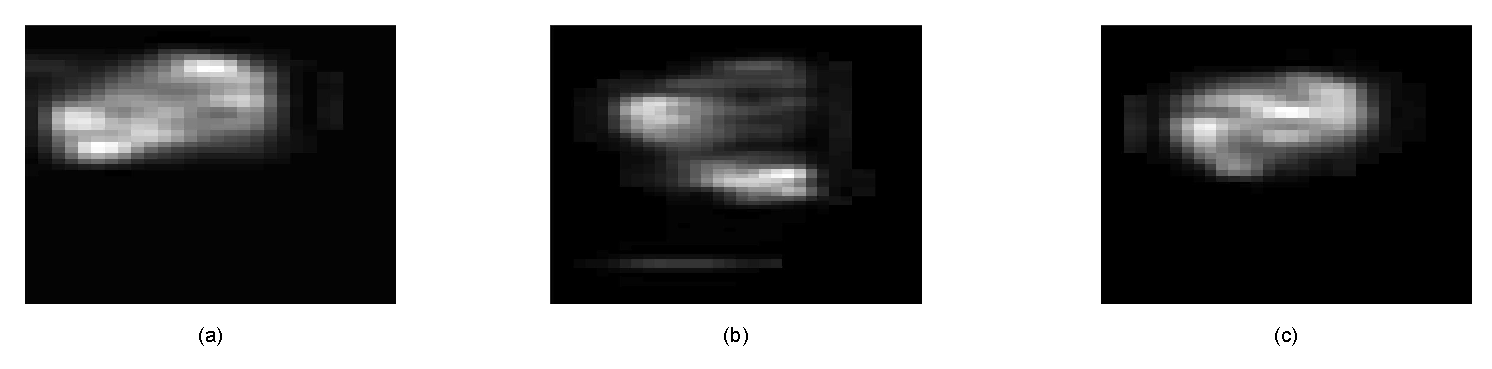
\includegraphics[width=8cm]{./figures/similar_steps.pdf}
	\caption{The transformed pressure sensor data corresponding to different moment of a step at different time. The heat maps (a) and (b) belong to the same person, (c) belongs to a different person.}
	\label{fig:similar_steps}
\end{figure}


% Paper Contribution
\subsection{Paper Contribution}
  In this paper, we introduce the idea of using the concept of transfer learning on a domain which is not easily visually interpretable. We carry out a shift procedure, which involves the shift from a domain which is not suitable for transfer learning to a domain on which the CNNs have been trained. This shift facilitates the use of transfer learning even for data which normally is not an ideal candidate for transfer learning. In order to show that such transformation is useful,  we extend the transfer learning methods on pressure sensor data. The raw sensor data is first transformed into a set of visual images and then used as an input dataset for a pre-trained convolutional network model. Thus, the core contributions of this paper are as follows:
\begin{itemize}
\item \textit{Modality transformation:} We transform non-interpretable data to the image domain and explore the effectiveness of deep neural networks. We observe that models which are pre-trained on the aesthetic and visually interpretable datasets like ImageNet, are powerful and accurate enough in terms of feature calculation that the artificially generated images are also recognized with high accuracy rates.

\item \textit{Unified feature extraction process:} Typically, the feature extraction process using conventional methods is customized for each unique application. In the case of sensor data, even with the same kind of sensors used for collecting the information, the feature extraction and data mining techniques vary depending on the target application of the data. The same pressure sensor has been used to cater to different applications \cite{cheng2016smart, SmartMat} but uses different feature extraction techniques. We provide a unified feature extraction process, which can be applied to the sensor data after conversion into the visual domain independent from its application.

\item \textit{Evaluation on pressure sensor data:} We evaluate our approach of modality transformation with pressure values of single steps as each person walks on a Smart-Mat \cite{SmartMat}, a fabric based real-time pressure force mapping system. The domain shift is carried out by transforming the pixel data values corresponding to the pressure exerted on the floor while walking (See Section \ref{pressuredata}), to the respective images. This information consisting of images serve as the input to pre-trained CNNs. With the application of our approach of modality transformation, we achieve a person identification accuracy of 87.66\% which significantly outperforms the state of the art (76.9 \%) (See Section \ref{sec:eval})

\end{itemize}


\section{A new construction method}

\label{secMainThm}

Let $X$ and $Y$ be complex manifolds and let $f:X\rightarrow Y$ be a surjective holomorphic map. Recall that a sufficient condition for the map $f$ to have isolated singularities is that the set of singular points of $f$ intersects every fibre of $f$ in a discrete set.

Before we proceed we fix some notation: For a set $M$ and subsets $A,B\subset M$ we will denote by $A\setminus B$ the set theoretic difference of $A$ and $B$. If $M=T^n$ is an $n$-dimensional torus then we will denote by $A-B=\left\{a-b\mid a\in A, b\in B\right\}$ the group theoretic difference of $A$ and $B$ with respect to the additive group structure on $T^n$. We will be careful to distinguish $-$ from set theoretic $\setminus$.

In this section we generalise the following result of Dimca, Papadima and Suciu to maps onto higher-dimensional tori.

\begin{theorem}[{\cite[Theorem C]{DimPapSuc-09-II}} ]
Let $X$ be a compact complex manifold and let $Y$ be a closed Riemann surface of genus at least one. Let $f: X\rightarrow Y$ be a surjective holomorphic map with isolated singularities and connected fibres. Let $\widehat{f}: \widehat{X}\rightarrow \widetilde{Y}$ be the pull-back of $f$ under the universal cover $p:\widetilde{Y} \rightarrow Y$ and let $H$ be the smooth generic fibre of $\widehat{f}$ (and therefore of $f$).

Then the following hold:
\begin{enumerate}
 \item $\pi_i(\widehat{X},H)=0$ for $ i \leq \mathrm{dim}H$;
 \item if $\mathrm{dim} H \geq 2$, then  $1\rightarrow \pi_1 H\rightarrow \pi_1 X\overset{f_{\ast}}\rightarrow \pi_1 Y\rightarrow 1$ is exact.
\end{enumerate}
\label{thmC'}
\end{theorem}

\subsection{Conjecture}
\label{secConjThmC}



Having isolated singularities yields strong restrictions on the topology of the fibres near the singularities. We will only make indirect use of these restrictions here, by applying Theorem \ref{thmC'}. For background on isolated singularities see \cite{Loo-84}.

\begin{conjecture}
Let $X$ be a compact connected complex manifold of dimension $n+k$ and let $Y$ be a $k$-dimensional complex torus or a Riemann surface of positive genus. Let $h: X\rightarrow Y$ be a surjective holomorphic map with connected generic fibre.

Let further $\widehat{h}:\widehat{X}\rightarrow \widetilde{Y}$ be the pull-back fibration of $h$ under the universal cover $p: \widetilde{Y}\rightarrow Y$ and let $H$ be the generic smooth fibre of $\widehat{h}$, or equivalently of $h$.

Suppose that $h$ has only isolated singularities. Then the following hold:
\begin{enumerate}
 \item $\pi_i(\widehat{X},H)=0$ for all $i\leq \mathrm{dim} H$;
 \item if, moreover, $\mathrm{dim} H\geq 2$ then the induced homomorphism $h_{\ast}: \pi_1 X\rightarrow \pi_1 Y$ is surjective with kernel isomorphic to $\pi_1 H$.
\end{enumerate}
\label{conjgenThmC}
\end{conjecture}

Conjecture \ref{conjgenThmC} is a generalisation of Theorem \ref{thmC'} to higher dimensions. It can be seen as a Lefschetz type result, since it says that in low dimensions the homotopy groups of the subvariety $H\subset \widehat{X}$ of codimension $n\geq 2$ coincide with the homotopy groups of $H$. The most classical Lefschetz type theorem is the Lefschetz Hyperplane Theorem (see \cite{GorMac-88} for a detailed introduction to Lefschetz type theorems). 

A potential proof strategy for Conjecture \ref{conjgenThmC} is presented in \cite{Llo-PhD}, but there are technical difficulties which we were not able to overcome yet. Here we will prove Theorem \ref{thmFiltVer}, which is a special case of Conjecture \ref{conjgenThmC}.


In fact we will prove the more general Theorem \ref{thmFiltVerGen} from which Theorem \ref{thmFiltVer} follows immediately. 

\subsection{Fibrelong isolated singularities}
\label{secFibrelongSingBriLlo}

To prove Theorem \ref{thmFiltVerGen} we make use of a generalisation of Theorem \ref{thmC'} which relaxes the conditions on the singularities of $h$.
 
\begin{definition}
 Let $X$, $Y$ be compact complex manifolds. We say that a surjective map $h: X\rightarrow Y$ has \textit{fibrelong isolated singularities} if it factors as
 \[
  \xymatrix{ X \ar[r]^g \ar[rd]^h & Z\ar[d]^f \\ & Y\\}
 \]
 where $Z$ is a compact complex manifold, $g$ is a regular holomorphic fibration, and $f$ is holomorphic with isolated singularities.
 \label{defAIS}
\end{definition}

For holomorphic maps with connected fibrelong isolated singularities, Bridson and the author proved

\begin{theorem}[{\cite[Theorem 2.2]{BriLlo-16}}]
\label{thm2}
Let $Y$ be a closed Riemann surface of positive genus and let $X$ be a compact K\"ahler manifold. Let $h:X\rightarrow Y$ be a surjective holomorphic map with connected generic (smooth) fibre $\overline{H}$.

If $h$ has fibrelong isolated singularities, $g$ and $f$ are as in Definition \ref{defAIS}, and $f$ has connected fibres of dimension $m\geq 2$, then the sequence 

\[  
1 \rightarrow \pi_1 \overline{H}\rightarrow \pi_1 X \overset{h_{\ast}}\rightarrow \pi_1 Y\rightarrow 1
\]
is exact.
\end{theorem}


We will also need the following proposition. Note that the hypothesis on $\pi_2 Z\to \pi_1F$  is automatically
satisfied if $\pi_1F$ does not contain a non-trivial normal abelian subgroup. This is the case, for example,
if $F$ is a direct product of hyperbolic surfaces.

\begin{proposition}[{\cite[Proposition 2.3]{BriLlo-16}}]
\label{prop1part2}
Under the assumptions of Theorem \ref{thm2}, if the map $\pi_2 Z\to \pi_1F$ associated to the fibration $g:X\to Z$ is trivial, then the long exact sequence induced by the fibration $F\hookrightarrow \overline{H}\rightarrow H$ reduces to a short exact sequence
\[
1\rightarrow \pi_1 F\rightarrow \pi_1 \overline{H}\rightarrow \pi_1 H\rightarrow 1.
\]
If, in addition, the fibre $F$ is aspherical, then $\pi_ i \overline{H} \cong \pi_i H \cong \pi_i X$ for $2\leq i \leq m - 1$.
\end{proposition}

\subsection{Restrictions on $h:X\rightarrow Y$ for higher-dimensional tori}
\label{sec:Restrictions}

Let $X$ be a compact complex manifold and let $Y$ be a complex torus of dimension $k$. Let $h: X\rightarrow Y$ be a surjective holomorphic map. Assume that there is a filtration
\[
 \left\{0\right\} \subset Y^0\subset Y^1 \subset \cdots \subset Y^{k-1}\subset Y^k=Y
\]
of $Y$ by complex subtori $Y^l$ of dimension $l$, $0\leq l \leq k$. Let $\pi_l: Y\rightarrow Y/Y^{k-l}$ be the canonical holomorphic projection.

Assume that the maps $h$ and $h_l=\pi_l\circ h: X\rightarrow Y/Y^{k-l}$ have connected fibres and fibrelong isolated singularities. In particular, there are compact complex manifolds $Z_l$ such that $h_l$ factors as
\[
 \xymatrix{ X \ar[r]^{g_l}\ar[rd]_{h_l} & Z_l\ar[d]^{f_l} \\ & Y/Y^{k-l}}.
\]
with $g_l$ a regular holomorphic fibration and $f_l$ surjective holomorphic with isolated singularities and connected fibres. Assume further that the smooth compact fibre $F_l$ of $g_l$ is connected and aspherical. We denote by $\overline{H}_l$ the connected smooth generic fibre of $h_l$ and by $H_l$ the connected smooth generic fibre of $f_l$. 

For a generic point $x^0=\left(x_1^0,\cdots, x_k^0\right)\in Y$ we claim that $x^{0,l}=x^{0,k}+Y^{k-l}\in Y/Y^{k-l}$ is a regular value of $h_l$ for $0\leq l \leq k$:  For $1\leq l \leq k$ there is a proper subvariety $V^l \subset Y/Y^{k-l}$ such that the set of critical values of $h_l$ is contained in $V^l$; any choice of $x^0$ in the open dense subset $Y \setminus \left(\cup_{l=1}^k \pi_l^{-1}(V^l)\right) \subset Y$ satisfies the assertion.
 
 The smooth generic fibres $\overline{H}_l=h_l^{-1}(x^{0,l})$ of $h_l$ form a nested sequence
 \[
  \overline{H}= \overline{H}_k\subset \overline{H}_{k-1}\subset \cdots \subset \overline{H}_0=X.
 \]

Consider the corestriction of $h_l$ to the elliptic curve $x^{0,l}+ Y^{k-l+1}/Y^{k-l}\subset Y/Y^{k-l}$. The map 
\[
 h_l|_{\overline{H}_{l-1}}: h_l^{-1}\left(x^{0,l}+ Y^{k-l+1}/Y^{k-l}\right)= h^{-1}\left(x^{0,k}+Y^{k-l+1}\right)=\overline{H}_{l-1}\rightarrow x^{0,l}+Y^{k-l+1}/Y^{k-l}
\]
is holomorphic surjective with fibrelong isolated singularities and connected smooth generic fibre $\overline{H}_l=h_l^{-1}(x^{0,l}+Y^{k-l})$.

Assume that the induced map $\pi_2 \overline{H}_{l-1}\rightarrow \pi_1 F_l$ is trivial for $1\leq l\leq k$. Then the following result holds:

\begin{theorem}
 Assume that $h:X\rightarrow Y$ has all the properties described in Paragraph \ref{sec:Restrictions} and that $n:= \mathrm{min}_{1\leq l \leq k} \mathrm{dim} H_l\geq 2$. Then the map $h$ induces a short exact sequence
 \[
  1\rightarrow \pi_1 \overline{H}\rightarrow \pi_1 X \stackrel{h_{\ast}}{\rightarrow} \pi_1 Y \cong \ZZ^{2k} \rightarrow 1
 \] 
and $\pi_i(\overline{H})\cong \pi_i (X)$ for $2\leq i \leq n-1$.
\label{thmFiltVerGen}
\end{theorem}

Note that Theorem \ref{thmFiltVer} is the special case of Theorem \ref{thmFiltVerGen} with $Z_l=X$ and $g_l=id_X$ for $1\leq l \leq k$.


\begin{proof}[Proof of Theorem \ref{thmFiltVerGen}]
 The proof uses an inductive argument reducing the statement to an iterated application of Theorem \ref{thm2} and Proposition \ref{prop1part2}.
 
Since $\mathrm{dim} H_l\geq n\geq 2$, Theorem \ref{thm2} and Proposition \ref{prop1part2} imply the restriction $h_l|_{\overline{H}_{l-1}}$ induces a short exact sequence
\begin{equation}
1\rightarrow \pi_1 \overline{H}_l \rightarrow \pi_1 \overline{H}_{l-1}\stackrel{h_{l\ast}}{\rightarrow} \pi_1 \left(x^{0,l}+ Y^{k-l+1}/Y^{k-l}\right) = \ZZ^2\rightarrow 1
\label{eqnSES1}
\end{equation}
and that $ \pi_i(\overline{H}_{l-1})\cong  \pi_ i(\overline{H}_l)$ for $2\leq i \leq \mathrm{dim} H_l-1$, where $1\leq l \leq k$. In particular, we obtain that $\pi_ i(\overline{H}_{l-1}) \cong \pi_i(\overline{H}_l)$ for $2\leq i \leq n-1$.
 
 Hence, we are left to prove that the short exact sequences in \eqref{eqnSES1} induce a short exact sequence
\[
1\rightarrow \pi_1 \overline{H} \rightarrow \pi_1 X\rightarrow \pi_1 Y=\ZZ^{2k}\rightarrow 1.
\]

For this consider the commutative diagram of topological spaces
\[
\xymatrix{
\overline{H} \ar@{^{(}->}[r] & X=\overline{H}_0=h_{k}^{-1}\left(x^{0,0}+ Y^k\right) \ar@{->>}[r] ^-{h} & x^{0,0}+ Y^k\\
\overline{H} \ar@{^{(}->}[r] \ar[u]^{=} & \overline{H}_1=h^{-1}\left(x^{0,1}+ Y^{k-1}\right) \ar@{->>}[r]^-{h} \ar@{^{(}->}[u] & x^{0,1}+ Y^{k-1} \ar@{^{(}->}[u] \\
  \ar[u]^{=} &  \ar@{^{(}->}[u] & \ar@{^{(}->}[u] \\
 \vdots & \vdots &\vdots \\
\overline{H} \ar@{^{(}->}[r] \ar[u]^{=} & \overline{H}_{k-1}=h_{k}^{-1}\left(x^{0,k-1}+ Y^1\right) \ar@{->>}[r]^-{h} \ar@{^{(}->}[u] & x^{0,k-1}+ Y^1 \ar@{^{(}->}[u] \\
\overline{H} \ar@{^{(}->}[r] \ar[u]^{=} & \overline{H}=\overline{H}_{k}=h_{k}^{-1}\left(x^{0,k}+ Y^0\right) \ar@{->>}[r]^-{h} \ar@{^{(}->}[u] & x^{0,k}+ Y^0 \ar@{^{(}->}[u] \\
} 
\]

This induces a commutative diagram of fundamental groups 
\begin{equation}
\xymatrix{
1\ar[r] & \pi_1 \overline{H} \ar@{^{(}->}[r] & \pi_1 X \ar@{->>}[r] ^-{h_{\ast}} & \pi_1(x^{0,0}+Y^{k})= \ZZ^{2k}\ar[r] &1\\
1\ar[r] & \pi_1 \overline{H} \ar@{^{(}->}[r] \ar[u]^{=} & \pi_1 \overline{H}_1 \ar@{->>}[r]^-{h_{\ast}} \ar@{^{(}->}[u] & \pi_1(x^{0,1}+Y^{k-1})=\ZZ ^{2k-2} \ar@{^{(}->}[u]\ar[r] &1 \\
 & \ar[u]^{=} &  \ar@{^{(}->}[u] & \ar@{^{(}->}[u] & \\
 & \vdots & \vdots &\vdots & \\
1\ar[r] & \pi_1 \overline{H} \ar@{^{(}->}[r] \ar[u]^{=} & \pi_1 \overline{H}_{k-1} \ar@{->>}[r]^-{h_{\ast}} \ar@{^{(}->}[u] & \pi_1(x^{0,k-1}+Y^1)=\ZZ ^2 \ar@{^{(}->}[u]\ar[r] &1 \\
1\ar[r] & \pi_1 \overline{H} \ar@{^{(}->}[r] \ar[u]^{=} & \pi_1 \overline{H} \ar@{->>}[r]^-{h_{\ast}} \ar@{^{(}->}[u] & \pi_1(x^{0,k}+Y^0)=1 \ar@{^{(}->}[u]\ar[r] &1 \\
}
\label{eqndiaggps}
\end{equation}
where injectivity of the vertical maps in the middle column follows from \eqref{eqnSES1}. The last two rows in this diagram are short exact sequences: The last row is obviously exact and the penultimate row is exact by \eqref{eqnSES1} for $l=k$.

We will now prove by induction (with $l$ decreasing) that the $l$-th row from the bottom
\[
1\rightarrow \pi_1 \overline{H} \rightarrow \pi_1 \overline{H}_l\rightarrow \pi_1(x^{0,l}+Y^{k-l})\rightarrow 1
\]
is a short exact sequence for $0\leq l\leq k$. 

Assume that the statement is true for $l$. We want to prove it for $l-1$. Exactness at $\pi_1\overline{H}$ follows from the sequence of injections $\pi_1 \overline{H}_l \hookrightarrow \pi_1 \overline{H}_{l-1}$.

For exactness at $\pi_1 (x^{0,l-1}+Y^{k-l+1})$ observe that, by the Ehresmann Fibration Theorem, the fibration $\overline{H}_{l-1}\rightarrow x^{0,l-1}+Y^{k-l+1}$ restricts to a locally trivial fibration $\overline{H}_{l-1}^*\rightarrow (x^{0,l-1}+Y^{k-l+1})^*$  with connected fibre $\overline{H}$ over the complement $(x^{0,l-1}+Y^{k-l+1})^*$ of the subvariety of critical values of $h$ in $x^{0,l-1}+Y^{k-l+1}$. Hence, the induced map $\pi_1 \overline{H}_{l-1}^*\rightarrow \pi_1 (x^{0,l-1}+Y^{k-l+1})^*$ on fundamental groups is surjective. Since the complements $\overline{H}_{l-1}\setminus \overline{H}_{l-1}^*$ and $(x^{0,l-1}+Y^{k-l+1})\setminus (x^{0,l-1}+Y^{k-l+1})^*$ are contained in complex analytic subvarieties of real codimension at least two, the induced map $\pi_1 \overline{H}_{l-1}\rightarrow \pi_1 (x^{0,l-1}+Y^{k-l+1})$ is surjective.

For exactness at $\pi_1 \overline{H}_{l-1}$ it is clear that $\pi_1 \overline{H}\leq \mathrm{ker}\left(\pi_1 \overline{H}_{l-1}\rightarrow \pi_1(x^{0,l-1}+Y^{k-l+1})\right)$. Hence, the only point that is left to prove is that $\pi_1 \overline{H}$ contains $$\mathrm{ker}\left(\pi_1 \overline{H}_{l-1}\rightarrow \pi_1(x^{0,l-1}+Y^{k-l+1})=\ZZ^{2k-2(l-1)}\right).$$
Let $g\in \mathrm{ker}\left(\pi_1 \overline{H}_{l-1}\stackrel{h_{\ast}}{\rightarrow} \pi_1(x^{0,l-1}+Y^{k-l+1}) \right)$. Then
\[
g\in \mathrm{ker}\left( \pi_1 \overline{H}_{l-1} \stackrel{h_{l\ast}}{\rightarrow} \pi_1 \left(x^{0,l}+ Y^{k-l+1}/Y^{k-l}\right)\right),
\]
since the map $h_{l\ast}$ factors through $h_{\ast}: \pi_1\overline{H}_{l-1}\rightarrow \pi_1(x^{0,l-1}+Y^{k-l+1})$.

By exactness of \eqref{eqnSES1} for $l$, this implies that there is $h\in \pi_1\overline{H}_l$ with $\iota_{l\ast}(h)=g$, where $\iota_l: \overline{H}_l\hookrightarrow \overline{H}_{l-1}$ is the inclusion map. It follows from commutativity of the diagram of groups \eqref{eqndiaggps} and injectivity of the vertical maps that $h\in \mathrm{ker}(\pi_1 \overline{H}_l\rightarrow \pi_1 (x^{0,l}+Y^{k-l}))$. The induction assumption now implies that $h\in \mathrm{Im} (\pi_1 \overline{H} \rightarrow \pi_1 \overline{H}_l)$.


Hence, by Induction hypothesis, $g\in \pi_1 \overline{H}$ and therefore the map $h|_{\overline{H}_{l-1}}$ does indeed induce a short exact sequence
\[
1\rightarrow \pi_1 \overline{H} \rightarrow \pi_1 \overline{H}_{l-1} \rightarrow \pi_1 Y^{k-l+1}\rightarrow 1.
\]

In particular, for $l=0$ we then obtain that $h$ induces a short exact sequence
\[
1\rightarrow \pi _1 \overline{H} \rightarrow \pi_1 X \rightarrow \pi_1 Y\rightarrow 1.
\]
\end{proof}

\begin{remark}
\label{rmkFiltVerGenWeak}
Note that in fact the proof of Theorem \ref{thmFiltVerGen} only requires that the corestrictions of the maps $h_l$ to $x^{0,l}+ Y^{k-l+1}/Y^{k-l}$ have isolated singularities and connected fibres. Thus, it suffices to check this weaker condition to apply Theorem \ref{thmFiltVerGen}. We will make use of this observation in Sections \ref{secExamples} and \ref{secExCombined}.
\end{remark}

\section{A class of higher dimensional examples}
\label{secExamples}

In this section we will construct a general class of examples of K\"ahler subgroups of direct products of surface groups arising as kernels of homomorphisms onto $\ZZ^{2k}$ for any $k\geq 1$. A subgroup $H\leq G_1 \times \dots \times G_r$ of a direct product of $r$ groups $G_i$ is called \textit{full} if all intersections $G_i\cap H:= \left(1\times \dots \times 1 \times G_i \times 1 \times \dots \times 1\right) \cap H$ are non-trivial, and \textit{subdirect} if $p_i(H)= G_i$ for all $1\leq i \leq r$, with $p_i: G_1 \times \dots \times G_r\to G_i$ the projection. We will give a more general discussion of full subdirect products of surface groups and their finiteness properties in Section \ref{secNotProd}.

Let $E=\CC/\Lambda$ be an elliptic curve, let $r\geq 3$ and let
\[
 \alpha _i: S_{\g_i}\rightarrow E
\]
be branched holomorphic coverings for $1\leq i \leq r$. 

Our groups will be the fundamental groups of the fibres of holomorphic surjective maps from the direct product $S_{\g_1}\times \cdots \times S_{\g_r}$ onto the $k$-fold direct product $E^{\times k}$ of $E$ with itself. For vectors $w_1,\cdots w_n\in \ZZ^k$ we will use the notation $\left(w_1\mid \cdots \mid w_n\right)$ to denote the $k\times n$-matrix with columns $w_i$. To construct these maps we make use of the following result

\begin{lemma}
Let $v_1=\left(v_{1,1},\cdots,v_{k,1}\right)^t,\cdots, v_r=\left(v_{1,r},\cdots,v_{k,r}\right)^t\in \ZZ^k$. Then the $\CC$-linear map $B=(v_1\mid v_2\mid \cdots \mid v_r)\in \ZZ^{k\times r}\subset \CC^{k\times r}$ descends to a holomorphic map
\[
 \overline{B}: E^{\times r}\rightarrow E^{\times k}.
\]
If, in addition, $r=k$ and $B\in \rm{GL}(k,\CC)\cap \ZZ^{k\times k}$ then $\overline{B}$ is a regular covering map. In particular, $\overline{B}$ is a biholomorphic automorphism of $E^{\times k}$ if $B\in \rm{GL}(k,\ZZ)$.
\label{lemAutkEll}
\end{lemma}

\begin{proof}
 It suffices to prove that $B$ preserves maps $\Lambda^{\times r}$ into $\Lambda^{\times k}$. For this let $\lambda_1,\lambda_2\in \CC$ be a $\ZZ$-basis for $\Lambda$ and denote by $\lambda_{1,i},\lambda_{2,i}$ the corresponding $\ZZ$-basis of the ith factor of $\Lambda ^ {\times r}$ and by $\lambda'_{1,j},\lambda'_{2,j}$ the corresponding $\ZZ$-basis of the jth factor of $\Lambda^{\times k}$. Then we have
 \[
  B \lambda_{i,j} = \sum _{l=1}^k v_{l,j} \lambda'_{i,l} \in \Lambda^{\times k} \mbox{    for   } 1\leq i \leq 2,\mbox{  }1\leq j \leq r
 \]
It follows that $B$ descends to a holomorphic map $\overline{B}:E^{\times r}\rightarrow E^{\times k}$. If $B\in \rm{GL}(k,\CC)\cap \ZZ^{k\times k}$ then $\overline{B}$ is a regular covering map, since $B$ is a local homeomorphism. If, in addition, $B\in \rm{GL}(k,\ZZ)$, then it is immediate that $\overline{B}$ and $\overline{B^{-1}}$ are mutual inverses.
\end{proof}



We say that a set of vectors $\mathcal{C}=\left\{v_1,\cdots, v_r\right\}\subset\ZZ^k$ has property 
\begin{enumerate}
\item[(P)] if there is $1\leq i_1 < \dots <i_k \leq r$ such that $\left\{v_{i_1},\dots,v_{i_k}\right\}$ is a $\ZZ$-basis for $\ZZ^k$ and any choice of $k$ vectors in $\mathcal{C}$ is linearly independent; and
\item[(P')] if $\mathcal{C}$ has property (P), and in addition $i_j=j$ and $\left\{v_1,\dots v_k\right\}$ is the standard basis for $\ZZ^k$.
\end{enumerate}

By Lemma \ref{lemAutkEll} for any set $\mathcal{C}=\left\{v_1,\cdots,v_r\right\}\subset \ZZ^k$ and $B=\left(v_1\mid \cdots \mid v_r\right)$ we can define a holomorphic map 
\[
h=\overline{B}\circ \left(\alpha_1,\cdots,\alpha_r\right)=\sum \limits_{i=1}^r v_i \cdot \alpha_i :S_{\g_1}\times \cdots \times S_{\g_r}\rightarrow E^{\times k}.
\]

We will be interested in maps $h$ for which the set $\mathcal{C}$ has property (P). Note that, after reordering factors and adjusting by a biholomorphic automorphism of $E^{\times k}$, say $A\in \rm{GL}(k,\ZZ)$, we may in fact assume that $\mathcal{C}$ has property (P') if it has property (P). 

The following result shows that such maps exist.

\begin{lemma}
 For all positive integers $r,k$ there is a set $\mathcal{C}=\left\{v_1,\cdots,v_r\right\}\subset \ZZ^k$ such that for all $1\leq i_1 <\dots <i_k\leq r$ the set $\left\{v_{i_1},\dots, v_{i_k}\right\}$ is linearly independent. Moreover, if $r\geq k$ we may assume that $\mathcal{C}$ satisfies property (P').
\label{lemLinIndep}
\end{lemma}

\begin{proof}
The proof is by induction on $r$. For $r=1$ the statement is trivial. Assume that for a positive integer $r$ we have a set $\mathcal{C}=\left\{v_1,\cdots, v_r\right\}\subset \ZZ^k$ of $r$ vectors with the property that for any $1\leq i_1<i_2<\cdots <i_k\leq r$ the subset $\left\{v_{i_1},\cdots,v_{i_k}\right\}\subset \mathcal{C}$ is linearly independent.

 Let $I$ be the set of all $(k-1)$-tuples $\mathbf{i}=(i_1,\cdots, i_{k-1})$ of integers $1\leq i_1<i_2<\cdots <i_{k-1}\leq r$. For $\mathbf{i}\in I$ denote by $W_{\mathbf{i}}=\mathrm{span}_{\CC}\left\{v_{i_1},\cdots, v_{i_{k-1}}\right\}$ the $\CC$-span of the linearly independent set $\left\{v_{i_1},\cdots, v_{i_{k-1}}\right\}$. Then $W=\bigcup\limits_{\mathbf{i}\in I} W_{\textbf{i}}$ is a finite union of complex hyperplanes in $\CC^k$ such that for any vector $v_{r+1}\in \ZZ^k\setminus W$ the set $\mathcal{C}\cup \left\{v_{r+1}\right\}$ has the desired property. The set $\ZZ^k\setminus W$ is nonempty, because $\ZZ^k\subset \CC^k$ is Zariski-dense in $\CC^k$.
 
 For $r\geq k$, choosing $\left\{v_1,\cdots,v_k\right\}$ to be the standard basis of $\CC^k$ ensures that property (P') is satisfied.
\end{proof}

\begin{remark}
 The proof of Lemma \ref{lemLinIndep} shows that we can choose any $m\leq r$ explicit vectors $v_1,\dots, v_m$ such that $\left\{v_1,\dots,v_m\right\}$ has property (P') and then complete to a set $\left\{v_1,\dots,v_r\right\}$ with property (P').
\end{remark}

Note that the proof of Lemma \ref{lemLinIndep} shows that the property (P') is in some sense a generic property.

The main result of this section is:

\begin{theorem}
 Let $1\leq k \leq r-2$ and let $\mathcal{C}\subset \ZZ^k$ be as defined above. Assume that $\mathcal{C}$ satisfies property (P'), and that $\alpha_1,\cdots,\alpha_k$ are surjective on fundamental groups. Then the smooth generic fibre $\overline{H}$ of $h$ is connected and its fundamental group fits into a short exact sequence
 \[
  1\rightarrow \pi_1 \overline{H} \rightarrow \pi_1 S_{\g_1}\times \cdots \times \pi_1 S_{\g_r}\stackrel{h_{\ast}}{\rightarrow} \pi_1 E^{\times k} = \ZZ^{2k}\rightarrow 1.
 \]
 Furthermore, $\pi_1 \overline{H}$ is an irreducible K\"ahler group of type $\mathcal{F}_{r-k}$ but not of type $\mathcal{F}_{r-k+1}$. In fact $\pi_j \overline{H} = 0$ for $2\leq j \leq r-k-1$.
 \label{thmExsGenClass}
\end{theorem}

Denote by $\pi_l : E^{\times k}\rightarrow \left\{0\right\} \times E^{\times l}$ the canonical projection onto the last $l$ factors and for a map $h$ satisfying the conditions of Theorem \ref{thmExsGenClass} let $h_l=\pi_l\circ h$. Due to the assumptions on $\mathcal{C}$ the map $h_l$ factors as $h_l= f_l\circ g_l$ for $1\leq l \leq k$ with
 \[
  f_l=\pi_l \circ \left(v_{k-l+1} \mid \cdots  \mid v_r\right)\circ(\a _{k-l+1},\cdots, \a _r):  S_{\g_{k-l+1}}\times \cdots \times S_{\g_r}\rightarrow Y^k/Y^{k-l}= \left\{0\right\} \times E^{\times l}  
 \]
 and
 \[
 g_l: S_{\g_1}\times \cdots \times S_{\g_r}\rightarrow  S_{\g_{k-l+1}} \times \cdots \times S_{\g_r}
 \]
 the canonical projection with fibre $F_l:= S_{\g_1}\times \cdots \times S_{\g_{k-l}}$, a product of closed hyperbolic surfaces (It follows from the fact that $v_1,\cdots, v_k\in \ZZ^k$ is a standard basis of $\ZZ^k$ that $h_l=f_l\circ g_l$ for $1\leq l \leq k$).

Theorem \ref{thmExsGenClass} will be a consequence of Theorem \ref{thmFiltVer} after checking that the maps $h$, $h_l$, $g_l$ and $f_l$ satisfy all necessary conditions.







The following is a natural and straight-forward generalization of \cite[Lemma 2.1]{Llo-16-II}.

\begin{lemma}
\label{lemNewConnFib}
 Let $X$ be a connected compact complex manifold, $E$ an elliptic curve and $f: X \rightarrow E$ a surjective holomorphic map. If there is a subgroup $A=\ZZ^2 \leq \pi_1 X$ such that $f_{\ast} A \leq \pi_1 E$ is a finite index subgroup and $f_{\ast} \pi_1 X = \pi_1 E$, then $f$ has connected fibres.
\end{lemma}

\begin{proof}
 Since $f$ is proper, by Stein factorisation, there is a compact Riemann surface $S$, such that $f$ factors as
 \[
 \xymatrix{ X \ar[r]^{h_1} \ar[rd]_f & S\ar[d] ^{h_2}\\ & E}
 \]
 where $h_1$ is holomorphic with connected fibres and $h_2$ is holomorphic and finite-to-one. In particular, $h_2$ is a (possibly ramified) covering map. 
 
 By assumption, the restriction $f_{\ast}|_A$ is injective. Thus, $h_{1,\ast} A\leq \pi_1 S$ defines a $\ZZ^2$-subgroup of $\pi_1S$. It follows that $S$ is an elliptic curve and $h_2: S\to E$ is an unramified cover. Surjectivity of $f_{\ast}: \pi_1 S\to \pi_1 E$ implies that $S=E$. Hence, $f$ has connected fibres.
\end{proof}


\begin{lemma}
\label{propConnGenExs}
  Under the assumptions of Theorem \ref{thmExsGenClass}, the maps $h$, $h_l$, $f_l$ and $g_l$, $1\leq l \leq k$ have connected fibres.
\end{lemma}
\begin{proof}
It suffices to consider the maps $f_l$, as the maps $g_l$ clearly have connected fibres and the connectedness of the fibres of the maps $h_l$ then follows from the identity $h_l=f_l\circ g_l$.

Choose a generic $x^0\in E^{\times k}=Y^k$ as in Section \ref{sec:Restrictions} and let $H_l=f_l^{-1}(x^{0,l})$, $\overline{H}_l=h_l^{-1}(x^{0,l})$ be the corresponding fibres. The proof is by induction on $l$.

First consider $l=1$. Then we have
\[
f_1= \pi_1 \circ \left(v_k\mid \dots \mid v_r\right) \circ \left(\alpha_k,\dots, \alpha_r\right): S_{\gamma_k}\times \dots \times S_{\gamma_r}\to Y^k/Y^{k-1}=\left\{0\right\} \times E.
\]
In particular, we have $f_1 =\sum_{j=k}^r v_{k,j}\cdot \alpha_j$. By assumption on $\mathcal{C}$, $r-k+1\geq 2$, and we have $v_{k,k}=1$ and $v_{k,j}\neq 0$ for $j\geq k$. Since $\alpha_k: S_{\gamma_k}\to E$ is surjective on fundamental groups, the same holds for $f_1$. Furthermore, the restriction $f_1|_{S_{\gamma_j}}$ defines a branched covering of $E$ for $k\leq j \leq r$. Hence, $f_{1,\ast}(\pi_1 S_{\gamma_j})\leq \pi_1 (\left\{0\right\} \times E)$ is a finite index subgroup for $k\leq j \leq r$. It follows that $f_1$ satisfies all conditions of Lemma \ref{lemNewConnFib} and therefore has connected fibres.

Let now $2\leq l \leq k$. By choice of $x^0$, the corestriction
\[
f_l|_{f_l^{-1}(x^{0,l}+ Y^{k-l+1}/Y^{k-l})}:f_l^{-1}(x^{0,l}+ Y^{k-l+1}/Y^{k-l}) \to x^{0,l}+ Y^{k-l+1}/Y^{k-l}
\]
has smooth generic fibre $H_l$. Since by definition $\pi_l(v_{k-l+1})=\left(\begin{array}{c}1\\0\\ \vdots\\ 0\end{array}\right)$, we obtain
\[
f_l^{-1}(x^{0,l}+ Y^{k-l+1}/Y^{k-l})=S_{\gamma_{k-l+1}}\times f_{l-1}^{-1}(x^{0,l-1})= S_{\gamma_{k-l+1}}\times H_{l-1},
\]
with $H_{l-1}$ smooth and connected by induction assumption.

Choose a basepoint $z_0\in S_{\gamma_{k-l+1}}$. By assumption on $\mathcal{C}$ the set $\pi_l(\left\{v_{k-l+2},\dots,v_r\right\})$ spans $\mathds{C}^l$. Thus, the map
\[
\sum_{j=k-l+2}^r \pi_l(v_j)\cdot \alpha_j: S_{\gamma_{k-l+2}}\times \dots \times S_{\gamma_r} \to Y^k/Y^{k-l} = \left\{0\right\}\times  E^{\times l}
\]
is a surjective holomorphic map. Thus, the same holds for the restriction $f_l|_{\left\{z_0\right\} \times S_{\gamma_{k-l+2}}\times \dots \times S_{\gamma_r}}$. It follows that 
\[
f_l|_{\left\{z_0\right\} \times H_{l-1}} : \left\{z_0\right\} \times H_{l-1}\to x^{0,l}+Y^{k-l+1}/Y^{k-l}
\]
is a surjective holomorphic map between compact complex manifolds and therefore $f_{l,\ast}(\pi_1 H_{l-1})\leq \pi_1 E$ is a finite index subgroup. On the other hand $\alpha_{k-l+1}$ is surjective on fundamental groups by assumption. Hence, $f_l|_{f_l^{-1}(x^{0,l}+ Y^{k-l+1}/Y^{k-l})}$ satisfies the assumptions of Lemma \ref{lemNewConnFib}. Therefore $f_l$ has connected smooth generic fibres.
\end{proof}




\begin{proposition}
Under the assumptions of Theorem \ref{thmExsGenClass} consider the filtration $Y^l=E^{\times l}\times \left\{0\right\}$ of $E^{\times k}$ where $\pi_l: E^{\times k}\rightarrow Y^k/Y^{k-l}= \left\{0\right\}  \times E^{\times l}$ is the projection onto the last $l$ coordinates. 
 
 Then the map $h$ satisfies the condition that $h_l=\pi_l\circ h$ has fibrelong isolated singularities for $0\leq l \leq k$. More precisely, the factorisation $h_l=f_l\circ g_l$ satisfies that $g_l$ is a regular fibration and $f_l$ has isolated singularities. Furthermore, the dimension of the smooth generic fibre $H_l$ of $f_l$ is r-k for $1\leq l \leq k$.
 
 \label{propIsolSingGen}
\end{proposition}

\begin{proof}
Recall that by definition of $f_l$ and $g_l$ we have $h_l=f_l\circ g_l$. The map $g_l$ is clearly a regular fibration. To see that the map $f_l$ has isolated singularities consider its differential
 \begin{equation}
  \D f_l = \left(\D \pi_l (v_{k-l+1})\cdot \mathrm{d} \a_{k-l+1},   \dots  ,\D\pi_l(v_r) \cdot \mathrm{d} \a_r\right).
 \label{eqnCritPt} 
 \end{equation}

Note that by definition of $\pi_l$ the vector $\D \pi_l(v_i)$ is the vector in $\ZZ^{l}$ consisting of the last $l$ entries of $v_i$. By property (P') any $k$ vectors in $\mathcal{C}$ form a linearly independent set. Furthermore we chose $\mathcal{C}$ such that $\mathcal{E}_1= \left\{v_1,\dots, v_k\right\}$ is the standard basis of $\ZZ^k$. This implies that the set
\[
\mathcal{C}_l = \left\{ \D \pi_l (v_{k-l+1}), \dots, \D\pi_l(v_r)\right\} \subset \ZZ^l
\]
also has property (P'). In particular, any choice of $l$ vectors in $\mathcal{C}_l$ forms a linearly independent set.

It follows from \eqref{eqnCritPt} that a point $(z_{k-l+1},\cdots, z_r)\in  S_{\g_{k-l+1}}\times \cdots \times S_{\g_r}$ is a critical point of $f_l$ if and only if $z_i$ is a critical point of $\alpha_i$ for at least $r-k+1$ of the $z_i$, where $k-l+1\leq i\leq r$.

Thus, the set of critical points $C_{f_l}$ of $f_l$ is the union $C_{f_l}=\bigcup \limits_{i\in I_l} B_{l,i}$ of a finite number of $(l-1)$-dimensional submanifolds $B_{l,i}\subset S_{\g_{k-l+1}}\times \cdots \times S_{\g_r}$ with the property that for every surface factor $S_{\g_j}$ of $S_{\g_{k-l+1}}\times \cdots \times S_{\g_r}$ the projection of $B_{l,i}$ onto $S_{\g_j}$ is either surjective or has finite image. Linear independence of any $l$ vectors in $\mathcal{C}_l$ implies that the restriction of $f_l$ to any of the $B_{l,i}$ is locally (and thus globally) finite-to-one. Hence, the intersection $C_{f_l}\cap H_{l,y}$ is finite for any fibre $H_{l,y}=f_l^{-1}(y)$, $y\in \left\{0\right\}\times E^{\times l}$. 

In particular, the map $f_l$ has isolated singularities. It follows immediately from the definition of $f_l$ that the smooth generic fibre $H_l$ of $f_l$ has dimension $r-(k-l)- l=r-k$.
\end{proof}


\begin{proof}[Proof of Theorem \ref{thmExsGenClass}]
 The proof follows from Theorem \ref{thmFiltVerGen}, Lemma \ref{propConnGenExs}  and Proposition \ref{propIsolSingGen}. Indeed, by Lemma \ref{propConnGenExs} and Proposition \ref{propIsolSingGen} combined with the fact that $F_l$ is a direct product of closed hyperbolic surfaces, all assumptions in Theorem \ref{thmFiltVerGen} are satisfied with $n=r-k$. Thus, the map $h$ induces a short exact sequence 
 \[
  1\rightarrow \pi_1 \overline{H}\rightarrow \pi_1 S_{\g_1}\times \cdots \times \pi_1 S_{\g_r} \stackrel{h_{\ast}}{\rightarrow} \pi_1 E^{\times k} \rightarrow 1 
 \]
 and isomorphisms $\pi_i \overline{H} \cong \pi_i (S_{\g_1}\times \cdots \times S_{\g_r})\cong 0$ for $2\leq i \leq r-k-1$.
 
 Since $\overline{H}$ is the smooth generic fibre of a holomorphic map, it is a compact complex submanifold and thus a compact projective submanifold of the projective manifold $S_{\g_1}\times \dots \times S_{\g_r}$.Thus, $\pi_1\overline{H}$ is a K\"ahler group (and in fact even a projective group). Furthermore, $\overline{H}$ can be endowed with the structure of a finite CW-complex.
 
 It follows that we can construct a classifying space $K(\pi_1\overline{H},1)$ from the finite CW-complex $\overline{H}$ by attaching cells of dimension at least $r-k+1$. Hence, there is a $K(\pi_1 \overline{H},1)$ with finitely many cells in dimension less than or equal to $r-k$. Thus, the group $\pi_1 \overline{H}$ is of type $\mathcal{F}_{r-k}$. Finally, by Lemma \ref{lemNotProdNotFr} in Section \ref{secNotProd}, the group $\pi_1 \overline{H}$ is irreducible and not of type $\mathcal{F}_{r-k+1}$.
\end{proof}

\begin{proof}[Proof of Theorem \ref{thmIntroA}]
Theorem \ref{thmIntroA} is now a direct consequence of Theorem \ref{thmExsGenClass}.
\end{proof}

 \begin{proof}[Proof of Theorem \ref{corthmIntroA}] 
 The only thing that does not follow immediately from Theorem \ref{thmIntroA} and its proof is that $\pi_1 \overline{H}$ is a full subdirect product. Considering the set $\mathcal{C}$ where $\left\{v_1,\dots,v_k\right\}$ is a standard basis of $\ZZ^k$ and $v_{k+1}=v_1+\dots +v_k$ we see that the complement $\mathcal{C}\setminus \left\{v_i\right\}$ of any vector contains a basis of $\ZZ^k$. Choosing $\alpha_{k+1}$ such that it induces an epimorphism on fundamental groups then assures that the restriction of $h_{\ast}$ to $\pi_1 S_{g_1}\times \dots \times \pi_1 S_{g_{i-1}}\times 1 \times \pi_1 S_{g_{i+1}}\times \dots \times \pi_1 S_{g_r}$ is surjective on fundamental groups for $1\leq i \leq r$ (see proof of Lemma \ref{lemNotProdNotFr} for more details on $h_{\ast}$). It follows that $\pi_1\overline{H}$ is subdirect. It is full, because the image of the restriction of $h_{\ast}$ to any factor is abelian.
 \end{proof}

\section{Examples from maps onto a product of two elliptic curves}
\label{secExCombined}
Note that the one-dimensional approach pursued in \cite{Llo-16-II} can not be used to obtain irreducible examples with finiteness properties as in Theorem \ref{corthmIntroA}. Indeed, choose any holomorphic map $h: S_{g_1}\times \dots \times S_{g_r}\to E$ and a base point $(z_1,\dots, z_r)\in S_{g_1}\times \dots \times S_{g_r}$. Then, for $2\leq m\leq r$, the restriction $h|_{\left\{(z_1,\dots,z_{m-1})\right\} \times S_{g_m}\times \left\{(z_{m+1},\dots,z_r)\right\}}$ is either trivial or surjective and thus the image $h_{\ast}(1\times \dots \times 1\times  \pi_1 S_{g_m}\times 1 \times \dots \times 1)\leq \pi_1 E$ is either trivial or a finite index subgroup. Therefore, if $h$ induces a short exact sequence on fundamental groups, then $\ker h_{\ast}$ is a product of finitely many surface groups and a group of the form constructed in \cite[Theorem 1.1]{Llo-16-II}. In particular, it is not irreducible unless it is of type $\mathcal{F}_{r-1}$ and not of type $\mathcal{F}_r$.

However, we can obtain irreducible examples covering all possible finiteness types using holomorphic maps to a product of two elliptic curves. This is achieved by combining the construction in Section \ref{secExamples} with Theorem \ref{thmFiltVerGen} and Remark \ref{rmkFiltVerGenWeak}. 

As before, we choose elements $v_1,\dots, v_r \in \ZZ^2$, as well as ramified covers $\alpha_i: S_{\g_i}\to E$ of an elliptic curve $E$ and define a holomorphic map 
\begin{equation}
h=\sum_{i=1}^r v_i\cdot \alpha_i : S_{\g_1}\times \dots \times S_{\g_r}\to E^{\times 2}.
\label{eqdefh}
\end{equation}
However, we will vary our choices of the $v_i$ to extend the range of finiteness properties of our examples.

Let $r\geq 4$, $m\geq 1$ and $r-m\geq 3$. Choose $v_1,\dots, v_m=\left( \begin{array}{c} 1\\ 0 \end{array} \right)$, $v_{m+1}=\left(\begin{array}{c} 0\\ 1 \end{array}\right)$ and $\left\{ v_{m+2}, \dots, v_r \right\}\subset \ZZ^2$ such that $\left\{ v_i, v_j\right\}$ are linearly independent for $m\leq i < j \leq r$. 

For the remainder of this section we denote $\mathcal{C}=\left\{v_1,\dots,v_r\right\}$ and $h$ the holomorphic map in \eqref{eqdefh} defined by this choice of $\mathcal{C}$. The main result of this section is:

\begin{theorem}
 Let $\mathcal{C} \subset \ZZ^2$ and $h$ be as defined above with $r\geq 4$, $m\geq 1$ and $r-m\geq 3$. Assume that $\alpha_m$ and $\alpha_{m+1}$ are surjective on fundamental groups. Then the smooth generic fibre $\overline{H}$ of $h$ is connected and its fundamental group fits into a short exact sequence
 \[
  1\to \pi_1 \overline{H} \to \pi_1 S_{\g_1}\times \dots \times S_{\g_r}\stackrel{h_{\ast}}{\to} \pi_1 E^{\times 2} = \ZZ^4 \to 1.
 \]
 Furthermore, $\pi_1 \overline{H}\leq \pi_1 S_{\g_1}\times \dots \times S_{\g_r}$ is an irreducible K\"ahler subgroup of type $\mathcal{F}_{r-m-1}$ but not of type $\mathcal{F}_{r-m}$. Moreover, $\pi_i \overline{H} =\left\{0\right\}$ for $2\leq i \leq r-m-2$.
 \label{thmExtendedRange}
\end{theorem}


As a consequence we obtain an alternative proof of Theorem \ref{corthmIntroA}. More precisely, we have:
\begin{corollary}
 For every $r\geq 4$, $r-1\geq k\geq 2$ and $\g_1,\dots,\g_r\geq 2$ there is an irreducible full subdirect K\"ahler subgroup $G\leq \pi_1 S_{\g_1}\times \dots \times \pi_1 S_{\g_r}$ of type $\mathcal{F}_k$ but not of type $\mathcal{F}_{k+1}$, which is the kernel of a homomorphism $\pi_1 S_{\g_1}\times \dots \times \pi_1 S_{\g_r}\to \ZZ^4$.
 \label{corExtendedRange}
\end{corollary}
\begin{proof}
We may choose $v_{m+1}=\left(\begin{array}{c}1\\1 \end{array}\right)$. Note that then the subgroups constructed in Theorem \ref{thmExtendedRange} are full subdirect, by the conditions imposed on $\mathcal{C}$ combined with the fact that the kernel of the induced map $\alpha_{i,\ast}: \pi_1 S_{\g_i} \to \pi_1 E = \ZZ^2$ is non-trivial for $1\leq i \leq r$ and their image is a finite index subgroup of $\ZZ^2$. 

For any $g\geq 2$ there is a branched covering $S_g\to E$ inducing an epimorphism on fundamental groups. Thus, Theorem \ref{thmExtendedRange} covers all $k<r-1$. The case $k=r-1$ is immediate from \cite[Theorem 1.1]{Llo-16-II}. 
\end{proof}

The proof of Theorem \ref{thmExtendedRange} is very similar to the proof of Theorem \ref{thmExsGenClass}. As in Section \ref{secExamples} we denote by $\pi_l : E^{\times 2}\to \left\{ 0 \right\} \times E^{\times l}$ the projection onto the last $l$ factors and by $h_l=\pi_l\circ h$ the composition. The map $h_l$ factors as $h_l = f_l \circ g_l$ for $1\leq l \leq 2$ with
\[
 f_2=\left(v_1\mid \dots \mid v_r \right) \circ \left(\alpha_1, \dots, \alpha_r \right) : S_{\g_1}\times \dots \times S_{\g_r}\to  E^{\times 2},
\]
\[
 g_2= S_{\g_1}\times \dots \times S_{\g_r} \to S_{\g_{1}}\times \dots \times S_{\g_r},
\]
\[
 f_1=\pi_1 \circ \left(v_{m+1}\mid \dots \mid v_r \right) \circ \left(\alpha_{m+1}, \dots, \alpha_r \right) : S_{\g_{m+1}}\times \dots \times S_{\g_r}\to  \left\{0\right\} \times E,
\]
and
\[
 g_1= S_{\g_1}\times \dots \times S_{\g_r} \to S_{\g_{m+1}}\times \dots \times S_{\g_r},
\]
where $g_1$ is the canonical projection with fibre $F_1=S_{\g_1}\times \dots \times S_{\g_m}$ a product of closed hyperbolic surfaces.

\begin{lemma}
\label{lemConnGenExsExt}
 Under the assumptions of Theorem \ref{thmExtendedRange}, the maps $h_i$, $f_i$ and $g_i$, $i=1,2$, have connected fibres.
\end{lemma}
\begin{proof}
 Since the maps $\alpha_m$ and $\alpha_{m+1}$ are surjective on fundamental groups, we see that by choice of $\mathcal{C}$, $r$ and $m$, the same argument as in the proof of Lemma \ref{propConnGenExs} shows connectedness of fibres.
\end{proof}



\begin{lemma}
 The map $f_1$ and the corestriction $f_2|_{f_2^{-1}(E\times \left\{e\right\})} : f_2^{-1}(E\times \left\{e\right\}) \to E\times \left\{ e \right\}$ have isolated singularities for all $e\in E$. 
 \label{lemIsSingExt}
\end{lemma}

Note that the map $f_2$ does not have isolated singularities. However, by Remark \ref{rmkFiltVerGenWeak} it suffices to show that the corestriction $f_2|_{f_2^{-1}(E\times \left\{e\right\})} : f_2^{-1}(E\times \left\{e\right\}) \to E\times \left\{ e \right\}$ has isolated singularities for all $e\in E$ to obtain the consequences of Theorem \ref{thmFiltVerGen}.

\begin{proof}
 For the map $f_1$ this follows by the same argument as in the proof of Proposition \ref{propIsolSingGen}. 
 
 The differential of $f_2$ is 
\begin{align*}
 Df_2 &= \left(v_1\cdot D\alpha_1 \dots v_r\cdot D\alpha_r\right)\\
      &= \left( \left( \begin{array}{c} 1\\ 0 \end{array}\right)\cdot D\alpha_1 \cdots \left(\begin{array}{c} 1\\ 0 \end{array} \right)\cdot D\alpha_m ~ v_{m+1} \cdot D\alpha_{m+1}\cdots v_r \cdot D \alpha_r\right).
\end{align*}

Due to our assumptions on $\mathcal{C}$, a point $z=(z_1,\dots,z_r)\in S_{\g_1}\times \dots \times S_{\g_r}$ is a critical point of $f_2$ if and only if at least one of the following holds
\begin{enumerate}
 \item $D\alpha_{m+1} (z_{m+1})=\dots = D\alpha_r (z_r)=0$;
 \item $D\alpha_1 (z_1)=\dots = D\alpha_m(z_m)= 0$ and at least $r-m-1$ of the $D\alpha_i(z_i)$ vanish for $i\geq m+1$.
\end{enumerate}

The locus of points satisfying (2) is a union of finitely many one-dimensional subvarieties of $S_{\g_1} \times \dots \times S_{\g_r}$ and it intersects each fibre of $f_2$ in at most finitely many points. Hence, these singularities are isolated for $f_2$ and thus for $f_2|_{f_2^{-1}(E\times \left\{e\right\})}$.

Observe that for the points $z\in f_2^{-1}(E\times \left\{e\right\})$ satisfying (1) but not (2), there exists at least one $i$ with $1\leq i\leq m$ such that $D\alpha_i(z_i)\neq 0$. The composition of $f_2|_{\left\{(z_1,\dots,z_{i-1})\right\} \times S_{\g_i} \times \left\{ (z_{i+1},\dots, z_r\right\}}$ with the projection onto the second factor of $E^{\times 2}$ is constant. Thus, $\left\{(z_1,\dots,z_{i-1})\right\} \times S_{\g_i} \times \left\{ (z_{i+1},\dots, z_r\right\} \subset f_2^{-1}(E\times \left\{e\right\})$ . In particular, $D\alpha_i(z_i)\neq 0$ implies that $D(f_2|_{f_2^{-1}(E\times \left\{e\right\})})(z)\neq 0$. 

Since $E\times \left\{e\right\}$ is one-dimensional, $z$ is not a critical point of the restriction $f_2|_{f_2^{-1}(E\times \left\{e\right\})}$. Hence, all critical points of $f_2|_{f_2^{-1}(E\times \left\{e\right\})}$ satisfy (2). It follows that $f_2|_{f_2^{-1}(E\times \left\{e\right\})}$ has isolated singularities.
\end{proof}

\begin{proof}[Proof of Theorem \ref{thmExtendedRange}]
By Lemma \ref{lemConnGenExsExt}, Lemma \ref{lemIsSingExt}, Remark \ref{rmkFiltVerGenWeak}, and the fact that $F_1$ is a direct product of surface groups, we can apply Theorem \ref{thmFiltVerGen}. We obtain that $h$ induces a short exact sequence
\[
 1\rightarrow \pi_1 \overline{H} \rightarrow \pi_1 S_{\g_1}\times \dots \times \pi_1 S_{\g_r}\stackrel{h_{\ast}}{\rightarrow} \pi_1 E^{\times 2}=\ZZ^4\rightarrow 1
\]
and $\pi_i \overline{H}=0$ for $2\leq i \leq r-m-2$. Hence, as in the proof of Theorem \ref{thmExsGenClass}, $\pi_1 \overline{H}$ is K\"ahler (and in fact projective) of type $\mathcal{F}_{r-m-1}$.

By definition, we obtain that $\phi=h_{\ast}$ is given by the surjective map
 \[
  h_{\ast}(g_1,\cdots,g_r)=\phi(g_1,\cdots,g_r)=\sum_{i=1}^r v_i\cdot \alpha_i(g_i) 
\in \pi_1 E^{\times 2} = (\ZZ^2)^2\cong \ZZ^4
\]
for $(g_1,\cdots,g_r)\in \pi_1 S_{\g_1}\times \cdots \times \pi_1 S_{\g_r}$. Assume that there is a finite index subgroup $H_1 \times H_2 \leq \ker \phi$. 

Since $\ker \phi$ is a full subdirect product (after possibly passing to finite index subgroups of the $\pi_1 S_{\g_i}$), we obtain that there is a partition of $\left\{1,\dots, r\right\}$ into two sets $\left\{i_1,\dots,i_t\right\}$ and $\left\{ i_{t+1},\dots, i_r\right\}$ such that $H_1 \leq \pi_1 S_{\g_{i_1}}\times \dots \times \pi_1 S_{\g_{i_t}}$ and $H_2 \leq \pi_1 S_{\g_{i_{t+1}}}\times \dots \times S_{\g_r}$ (because non-trivial elements of surface groups have cyclic centralizers).

Thus, for any element $(x_{i_1},\dots,x_{i_r})\in H_1\times H_2\leq \Gamma_{\g_{i_1}}\times \dots \times \Gamma_{\g_{i_r}}$, we have $(x_{i_1},\dots,x_{i_t},1,\dots,1)\in H_1\times 1 \leq \ker \phi$ and $(1,\dots,1,x_{i_{t+1}},\dots,x_{i_r})\leq 1 \times H_2 \leq \ker \phi$. By our assumptions on $\mathcal{C}$ at least one of $\left\{v_{i_1},\dots,v_{i_t}\right\}$ and $\left\{v_{i_{t+1}},\dots,v_{i_r}\right\}$ contains a pair of linearly independent vectors, say $\left\{v_{i_{t+1}},v_{i_{t+2}}\right\}$ are linearly independent.

Let $A\leq \ZZ^4 = (\ZZ^2)^2$ be the finite index subgroup with $A= \mathrm{Im} \left( v_{i_{t+1}}\cdot\alpha_{i_{t+1},\ast} + v_{i_{t+2}}\cdot \alpha_{i_{t+2},\ast}\right)$. Then for any element $x_{i_1}\in \Lambda_{i_1}$ of the finite index subgroup $\Lambda_{i_1}:=\left( v_{i_1} \cdot \alpha_{i,\ast}\right)^{-1}(A)\unlhd \Gamma_{\g_{i_1}}$ there is $(x_{i_{t+1}},x_{i_{t+2}})\in \Gamma_{\g_{i_{t+1}}}\times \Gamma_{\g_{i_{t+2}}}$ with $(x_{i_1},1,\dots,1,x_{i_{t+1}},x_{i_{t+2}},1,\dots,1)\in \ker \phi$. Hence, the intersection $\ker \phi \cap \left(\Gamma_{\g_{i_1}}\times \Gamma_{\g_{i_{t+1}}}\times \Gamma_{\g_{i_{t+2}}}\right)$ projects to a finite index subgroup of $\Gamma_{\g_{i_1}}$. Since $H_1\times H_2\leq \ker \phi$ is a finite index subgroup, the same is true for the projection of the intersection $\left(H_1\times H_2\right) \cap \left(\Gamma_{\g_{i_1}}\times \Gamma_{\g_{i_{t+1}}}\times \Gamma_{\g_{i_{t+2}}}\right)$ to $\Gamma_{\g_{i_1}}$. Thus, $H_1\times 1 $ contains a finite index subgroup of $\Gamma_{\g_{i_1}}$. This is impossible, because $\ker \alpha_{i_1,\ast}\leq \Gamma_{i_1}$ has infinite index. It follows that $\ker \phi$ is irreducible.

Finally observe that $v_1=\dots=v_m=\left(\begin{array}{c} 1\\ 0 \end{array}\right)$, implies that the image $\phi(\Gamma_{\g_1}\times \dots \times \Gamma_{\g_m})\cong \ZZ^2 \leq \ZZ^4=\mathrm{Im} \phi$ is not a finite index subgroup. Thus, the group $\ker \phi$ is not of type $\mathcal{F}_{r-m}$, by Corollary \ref{propCoNilpFm} below.
\end{proof}

\begin{remark}
 Note that one could also apply the converse direction of Theorem \ref{thmKochlVSPk} to obtain that the groups constructed in Theorem \ref{thmExsGenClass} and Theorem \ref{thmExtendedRange} have finiteness type $\mathcal{F}_{r-k}$ (respectively $\mathcal{F}_{r-m-1}$). However, the proof we give actually provides the stronger result that in fact classifying spaces for our examples can be constructed from compact K\"ahler manifolds by attaching only cells of dimension larger than $r-k$ (respectively $r-m-1$).
\end{remark}

\begin{remark}
\label{remNotIsom}
  By \cite[Theorem C(3)]{BriHowMilSho-13} a group $G$ which is a full subdirect product $G\leq \L_1\times \dots \times \L_r$ of non-abelian limit groups $\L_i$ uniquely determines the $\L_i$ (up to order). Assume that $G_1,G_2\leq G$ are two finite index subgroups which are full subdirect products $G_i\unlhd \L_{1,i}\times \dots \times \L_{r,i}$ with $\L_{j,i}\leq \L_j$, finite index subgroups such that $A_i=(\L_{1,i}\times \dots \times \L_{r,i})/G_i$ is free abelian, where $1\leq j\leq r$, $i=1,2$. It is not hard to see that then $A_1\cong A_2$. As a consequence we see that the examples constructed in this section are not isomorphic to the examples in the previous section for $m\geq 2$ (not even virtually).
\end{remark}




\begin{remark}
 The construction described in this section generalises to epimorphisms to $\ZZ^{2k}$ for any $k\geq 2$. This produces irreducible coabelian K\"ahler subgroups of a direct product of $r\geq 3$ surface groups of type $\mathcal{F}_m$, not $\mathcal{F}_{m+1}$ for $2\leq m \leq r-k$. The same arguments as in Remark \ref{remNotIsom} allow us to show that two irreducible groups obtained in this way are not isomorphic if they have different coabelian ranks, even if they have the same finiteness properties. For simplicity of notation, we restricted ourselves to the case $k=2$ in our explicit computations.
\end{remark}



\section{Finiteness properties and irreducibility}
\label{secNotProd}

In this section we want to determine the precise finiteness properties of our examples and prove that they are irreducible.

 Let $H\leq G = G_1\times\dots \times G_r$ be a subgroup of a direct product of groups $G_1,\cdots, G_r$. For every $1\leq i_1 < \dots < i_k \leq r$ denote by $p_{i_1,\cdots,i_k}: G \rightarrow G_{i_1}\times \dots \times G_{i_k}$ the canonical projection. We say that the group $H$ \textit{virtually surjects onto $k$-tuples} if for every $1\leq i_1 < \cdots < i_k\leq r$ the group $p_{i_1,\cdots, i_k}(H)$ has finite index in $G_{i_1}\times \dots \times G_{i_k}$. We say that $H$ is \textit{surjective on $k$-tuples} if for every $1\leq i_1 < \cdots < i_k\leq r$ we have equality $p_{i_1,\cdots,i_k}(H)=G_{i_1}\times \dots \times G_{i_k}$. We say that $H$ is \textit{virtually surjective on pairs} (VSP) if $H$ virtually surjects onto $2$-tuples.
 
 We further say that $H$ is \textit{coabelian of rank $k$} if there is an epimorphism $\phi: G_1\times \dots \times G_r\to \ZZ^k$ such that $H=\ker \phi$, and that $H$ is virtually coabelian of rank $k$ if there are finite index subgroups $H_0\leq H$ and $G_{i,0}\leq G_i$ such that $H_0\leq G_{1,0}\times \dots \times G_{r,0}$ is coabelian of rank $k$. It is not hard to see that the coabelian rank of $H$ is invariant under passing to finite index subgroups (see also Remark \ref{remNotIsom}).

For subgroups of direct products of limit groups, a close relation between their finiteness properties and virtual surjection to $k$-tuples has been observed (see \cite{BriHowMilSho-13},\cite{Koc-10}, also \cite{Kuc-14}). In fact if a subgroup $H\leq G_1\times \cdots \times G_r$ of a direct product of finitely presented groups is subdirect (i.e. surjects onto 1-tuples) then $H$ is finitely generated; and if it is VSP then $H$ is itself finitely presented \cite[Theorem A]{BriHowMilSho-13}. The converse is not true in general; it is true though if $G_1,\cdots, G_r$ are (non-abelian) limit groups and $H$ is full subdirect \cite[Theorem D]{BriHowMilSho-13}.

More generally it is conjectured \cite{Koc-10} that, for $G_1,\cdots, G_r$ non-abelian limit groups and $H\leq G_1\times \cdots \times \times G_r$ a full subdirect product, the following are equivalent:
\begin{enumerate}
 \item $H$ is of type $\mathcal{F}_k$;
 \item $H$ virtually surjects onto $k$-tuples.
\end{enumerate}  

Kochloukova proved that (1) implies (2) and gave conditions under which (2) implies (1).

\begin{theorem}[{Kochloukova \cite[Theorem C]{Koc-10}}]
 For $r\geq 1$ let $G_1, \dots , G_r$ be non-abelian limit groups, let $H\leq G_1\times \dots \times G_r$ be a full subdirect product, and let $2\leq k \leq r$. If $H$ is of type $\mathcal{F}_k$ then $H$ virtually surjects onto $k$-tuples. The converse is true if $H$ is virtually coabelian.
 \label{thmKochlVSPk}
\end{theorem}

Note that in Kochloukova's statement of Theorem \ref{thmKochlVSPk} the condition is that $H$ has the homological finiteness type $\rm{FP}_k(\mathds{Q})$. By \cite[Corollary E]{BriHowMilSho-13} this is however equivalent to type $\mathcal{F}_k$ for subgroups of direct products of limit groups. In general we only have that $\mathcal{F}_k$ implies $\rm{FP}_k(\mathds{Q})$ (see for instance \cite[Section 8.2]{Geo-08}).

\begin{remark}
It should be noted that the examples constructed in Theorem \ref{thmExtendedRange} are in some sense degenerate examples of type $\mathcal{F}_{r-m-1}$, but not of type $\mathcal{F}_{r-m}$, as the only $(r-m)$-tuple in $\pi_1 S_{\gamma_1}\times \dots \times S_{\gamma_r}$ onto which $\pi_1 \overline{H}$ does not (virtually) surject is $\pi_1 S_{\gamma_{m+1}}\times \dots \times \pi_1 S_{\gamma_r}$.
\end{remark}

We shall need the following auxiliary result which is a consequence of Theorem \ref{thmKochlVSPk}.

\begin{lemma}
 Let $G_1,\cdots, G_r$ be groups and $Q$ be a finitely generated abelian group. Let $\phi: G_1 \times \dots \times G_r \rightarrow Q$ be an epimorphism. Assume that the subgroup $H=\ker \phi \leq G_1\times \dots \times G_r$ virtually surjects onto $m$-tuples. Then the group $\phi( G_{i_1}\times \cdots \times G_{i_{r-m}})\leq Q$ is a finite index subgroup of $Q$ for every $1\leq i_1 < \dots < i_{r-m}\leq r$.
 
 Under the stronger assumption that $H$ surjects onto $m$-tuples, the restriction  of $\phi$ to $G_{i_1}\times \dots \times G_{i_{r-m}}$ is surjective for all $1\leq i_1 < \dots < i_{r-m}\leq r$.
\label{lemSurjComp}
\end{lemma}

\begin{proof}
 Assume that $H$ virtually surjects onto $m$-tuples. Consider a product $G_{i_1}\times \dots \times G_{i_{r-m}}$ of $r-m$ factors. We may assume that $i_j=j$.
 
Let $g\in Q$ be an arbitrary element. By surjectivity of $\phi$ there exist elements $h_1\in G_1\times \cdots \times G_{r-m}$ and $h_2 \in G_{r-m+1}\times \cdots \times G_r$ such that $g=\phi(h_1)\cdot \phi(h_2)$. Since $H$ virtually surjects onto $m$-tuples there is $k\geq 1$ such that $h_2^k\in p_{r-m+1,\cdots,r}(H)$. Hence, there is $\overline{h}_1\in G_{1}\times \cdots \times G_{r-m}$ such that $\overline{h}_1 \cdot h_2^k\in H=\ker \phi$. In particular it follows that $\phi(h_2^k)=\phi((\overline{h}_1)^{-1})$. As a consequence we obtain that $g^k = \phi(h_1)^k \cdot \phi(h_2)^k = \phi(h_1)^k\cdot \phi((\overline{h}_1)^{-1})\in \phi(G_{1}\times \cdots \times G_{r-m})$.

We proved that the abelian group $Q/\phi(G_{1}\times \cdots \times G_{r-m})$ has the property that each of its elements is torsion. This implies that $Q/\phi(G_{1}\times \cdots \times G_{r-m})$ is finite and thus $\phi(G_{1}\times \cdots \times G_{r-m})$ is a finite index subgroup of $Q$.

The second part follows immediately, since we can choose $k=1$ in the proof if H surjects onto $G_{r-m+1}\times \dots \times G_r$.
\end{proof}


\begin{corollary}
 Let $\phi: \L_1 \times \cdots \times \L_r\rightarrow Q$ be an epimorphism, where $\L _1,\cdots,\L_r$ are non-abelian limit groups and $Q$ is a finitely generated abelian group. If $\ker \phi$ is a full subdirect product of type $\mathcal{F}_m$ then the image $\phi(\L_{i_1} \times \cdots \times \L_{i_{r-m}})\leq Q$ is a finite index subgroup of $Q$ for all $1\leq i_1< \cdots < i_{r-m}\leq r$.
 \label{propCoNilpFm}
\end{corollary}
\begin{proof}
This is a direct consequence of Lemma \ref{lemSurjComp} and Theorem \ref{thmKochlVSPk}.
\end{proof}



As another consequence of Theorem \ref{thmKochlVSPk} we obtain. 

\begin{lemma}
 Let $G\leq \L_1\times \dots \times \L_r$ be a full subdirect product of $r$ non-abelian limit groups $\L_i$ of type $\mathcal{F}_m$ which is virtually a product $H_1\times H_2$. Then, after possibly reordering factors, there is $1\leq s \leq r$ such that $H_1\leq \L_1 \times \dots \times \L_s$ and $H_2\leq \L_{s+1}\times \dots \times \L_r$. Furthermore one of the following holds:
 \begin{enumerate}
  \item at least one of $H_1$ and $H_2$ is of type $\mathcal{F}_{\infty}$;
  \item $G$ virtually surjects onto at least one $2m$-tuple.
 \end{enumerate}
 \label{lemmNotProdKochl}
\end{lemma}
\begin{proof}
 Centralizers of elements in limit groups are infinite cyclic. Hence, subdirectness of $G$ implies that there is $1\leq s \leq r$ such that $H_1\leq \L_1 \times \dots \times \L_s$ and $H_2\leq \L_{s+1}\times \dots \times \L_r$. Theorem \ref{thmKochlVSPk} implies that $G$ and thus $H_1\times H_2$ virtually surjects onto $m$-tuples in $\L_1 \times \dots \times \L_r$. If either $s\leq m$ or $r-s\leq m$, say $s\leq m$, then $H_1 \times H_2$ surjects onto a finite index subgroup of $\L_1 \times \dots \times \L_s$. However, the projection is isomorphic to $H_1$. Thus, $H_1$ is a finite index subgroup of $\L_1 \times \dots \times L_s$ and therefore of type $\mathcal{F}_{\infty}$.
 
 Now assume that $s, ~ r-m > m$. In this case $H_1 \times H_2 $ virtually surjects onto $m$-tuples in $\L_1 \times \dots \times \L_s$ and $\L_{s+1}\times \dots \times \L_{r}$. Factoring the projections onto such $m$-tuples through the projections onto $\L_1 \times \dots \times \L_s$ and $\L_{s+1}\times \dots \times \L_r$, we see that $H_1\leq \L_1 \times \dots \times \L_s$ and $H_2\leq \L_{s+1}\times \dots \times \L_r$ also virtually surject onto $m$ tuples. Thus, $H_1\times H_2$ virtually surjects onto at least one $2m$-tuple and the same holds for $G$. 
\end{proof}

\begin{remark}
Note that Lemma \ref{lemmNotProdKochl} can also be applied to full subgroups $G\leq \L_1\times \dots \times \L_r$, after replacing the $\L_i$ by the projections of $G$ to $\L_i$ and $G$ by the quotient $G/Z(G)$ by the center $Z(G)$, since $G/Z(G)$ and $G$ have the same finiteness type by \cite[Proposition 2.7]{Bie-81}.
\end{remark}



We shall also need the following result by Kuckuck.

\begin{proposition}[{\cite[Corollary 3.6]{Kuc-14}}]
 Let $G\leq \L_1 \times \cdots \times \L_r$ be a full subdirect product of a direct product of $r$ non-abelian limit groups $\L_i$, $1\leq i \leq r$. If $G$ virtually surjects onto $m$ tuples for $m> \frac{r}{2}$ then $G$ is virtually coabelian. In particular, $G$ is virtually coabelian if $G$ is of type $\mathcal{F}_m$. 
 
 More precisely, we have that in either case there exist finite index subgroups $\L'_i\leq \L_i$, a free abelian group $A$ and a homomorphism
 \[
 \phi: \L'_1\times \cdots \times \L'_r \rightarrow A
 \]
such that $\ker \phi\leq G$ is a finite index subgroup.
\label{thmCoNilpFm}
\end{proposition}

We will require the following consequence of Theorem \ref{thmKochlVSPk} and Proposition \ref{thmCoNilpFm}:
\begin{corollary}
\label{corFinPropsProjFactors}
 Let $r\geq 1$ and let $G\leq \L_1 \times \cdots \times \L_r$ be a full subdirect product of non-abelian limit groups $\L_i$, $1\leq i \leq r$. Assume that $G$ is of type $\mathcal{F}_m$ with $m\geq 0$. For $k\geq 0$ with $m>\frac{k}{2}$ and $1\leq i_1 < \dots < i_k\leq r$ the projection $p_{i_1,\cdots,i_k}(G)\leq \L_{i_1}\times \dots \times \L_{i_k}$ is of type $\mathcal{F}_m$.
\end{corollary}
\begin{proof}
 By Theorem \ref{thmKochlVSPk} the group $G\leq \L_1 \times \cdots \times \L_r$ virtually projects onto $m$-tuples. Hence, the projection $\overline(G):=p_{i_1,\cdots,i_k}(G)\leq \L_{i_1}\times \cdots \times \L_{i_k}$ is full subdirect and virtually surjects onto $m$-tuples with $m> \frac{k}{2}$. By Proposition \ref{thmCoNilpFm} $\overline{G}$ is virtually coabelian in $\L_{i_1}\times \cdots \times \L_{i_k}$. Hence, the subgroup $\overline{G}\leq \L_{i_1}\times \cdots \times \L_{i_k}$ is full subdirect, virtually coabelian, and virtually projects onto $m$-tuples. The converse direction of Theorem \ref{thmKochlVSPk} then implies that $\overline{G}$ is of type $\mathcal{F}_m$.
\end{proof}

As a consequence of the results in this section we can determine the precise finiteness properties and irreducibility of the groups arising from our construction in Theorem \ref{thmExsGenClass}.
\begin{lemma}
 Under the assumptions of Theorem \ref{thmExsGenClass} and with the same notation, let  $\phi=h_{\ast}: \pi_1 S_{\g_1}\times \cdots \times \pi_1 S_{\g_r}\rightarrow \pi_1 E^{\times k}$ be the induced epimorphism on fundamental groups. Then $\ker \phi \cong \pi_1 \overline{H}$ is irreducible of type $\mathcal{F}_{r-k}$ and not of type $\mathcal{F}_{r-k+1}$.
 \label{lemNotProdNotFr}
\end{lemma}
\begin{proof}
 By the proof of Theorem \ref{thmExsGenClass} we know that $\ker \phi$ is of type $\mathcal{F}_{r-k}$. Hence, we only need to proof that $\ker \phi$ is not of type $\mathcal{F}_{r-k}$ and that $\ker \phi$ has no finite index subgroup which is a direct product of two non-trivial groups.
 
 As in the proof of Theorem \ref{thmExtendedRange} we have
 \[
  \phi(g_1,\cdots,g_r)=\sum_{i=1}^r v_i\cdot \alpha_i(g_i) \in (\pi_1 E)^{\times k}\cong (\ZZ^2)^{k}\cong \ZZ^{2k}
 \]
 for $(g_1,\cdots,g_r)\in \pi_1 S_{\g_1}\times \cdots \times \pi_1 S_{\g_r}$.
 
 Since the maps $\alpha_i$ are finite sheeted branched coverings, the image $\alpha_{i,\ast}(\pi_1S_{\g_i})\leq \pi_1 E$ is a finite index subgroup for $1\leq i \leq r$. The assumption that the $v_i$ satisfy property (P') implies that the image $\phi(\pi_1 S_{\g_{i_1}}\times \cdots \times \pi_1 S_{\g_{i_k}})\leq \pi_1 E^{\times k}$ of any $k$ factors is a finite index subgroup of $\pi_1 E^{\times k}\cong \ZZ^{2k}$, $1\leq i_1 < \cdots < i_k\leq r$.
 
 
 Since we have $r\geq k+2$ factors and any $k$ factors map to a finite index subgroup of $\pi_1 E^{\times k}$ the kernel of 
\[ 
 \phi_0=\phi|_{\L_1\times \cdots \times \L_r}: \L_1 \times \cdots \times \L_r\rightarrow \pi_1 E^{\times k}.
\]
is subdirect, after passing to finite index subgroups $\L_i\leq \pi_1 S_{\g_i}$. Note that the image $\rm{im} \phi_0\leq \pi_1 E^{\times k}$ is a finite index subgroup, thus isomorphic to $\ZZ^{2k}$, and that $\ker \phi_0 \leq \ker \phi$ is a finite index subgroup. The intersection $\L_i \cap \ker \phi_0\unlhd \L_i$ is a non-trivial normal subgroup of infinite index in $\L_i$, since $\phi(\L_i)\cong \ZZ^2$. Thus, $\ker \phi_0$ is a full subdirect product of $\L_1 \times \cdots \times \L_r$.
 
 Since the image of the restriction of $\phi_0$ to any factor $\L_i$ is isomorphic to $\ZZ^2$, the image of the restriction of $\phi$ to any $k-1$ factors $\L_{i_1}\times \cdots \times \L_{i_{k-1}}$ ($1\leq i_1 < \cdots < i_{k-1}$) is isomorphic to $\ZZ^{2(k-1)}$ (by the same argument as for $k$ factors). In particular, $\phi(\L_{i_1}\times \cdots \times \L_{i_{k-1}})$ is not a finite index subgroup of the image ${\rm{im}} \phi_0\cong \ZZ^{2k}$. By Corollary \ref{propCoNilpFm}, $\ker \phi_0$ and therefore its finite extension $\ker \phi \geq \ker \phi_0$ cannot be of type $\mathcal{F}_{r-k+1}$. 
 
 Assume that there is a finite index subgroup $H_1 \times H_2 \leq \ker \phi$ which is a product of two non-trivial groups $H_1$ and $H_2$. By Lemma \ref{lemmNotProdKochl} we may assume that (after reordering factors) $H_1 \leq \pi_1 S_{\g_1} \times \cdots \times \pi_1 S_{\g_s}$, $H_2 \leq \pi_1 S_{\g_{s+1}}\times \cdots \pi_1 S_{\g_r}$, for some $1\leq s \leq r-1$. If $H_1$ (or $H_2$) is of type $\mathcal{F}_{\infty}$ then it follows from \cite[Theorem A]{BriHowMilSho-09} that $H_1$ is virtually a product of finitely generated subgroups $\G_i \leq \pi_1 S_{\g_i}$, $1\leq i \leq s$. Since $\ker \phi_0$ is subdirect in $\L_1 \times \cdots \times \L_r$ and $\ker \phi_0 \cap (H_1\times H_2)\leq \ker \phi_0$ has finite index, the $\G_i$ must be finite index subgroups of the $\pi_1 S_{\g_i}$. This contradicts that the restriction of $\phi$ to any finite index subgroup of $\pi_1 S_{\g_i}$ has infinite image. Hence, by Lemma \ref{lemmNotProdKochl}, $\ker \phi$ virtually surjects onto at least one $2(r-k)$-tuple. However, the genericity condition (P') satisfied by $\mathcal{C}$ implies that $\ker \phi$ does not surject onto any $(r-k+1)$-tuple (the argument is the same as in the proof of Lemma \ref{lemSurjComp}). In particular $\ker \phi$ is irreducible.
\end{proof}

\begin{addendum}
 Note that the proof of Lemma \ref{lemNotProdNotFr} also shows that if we consider $\phi$ where the set $\mathcal{C}$, as defined in Theorem \ref{thmExsGenClass}, does not have the generic property described in Lemma \ref{lemLinIndep} then $\ker \phi$ must have finiteness type less than $\mathcal{F}_{r-k}$. In fact it shows that the finiteness type of $\ker \phi$ is at most $\mathcal{F}_{r-l}$ where $l-1$ is the size of a maximal subset of $\mathcal{C}$ which does not form a basis of $\CC^k$. Indeed we made use of this observation to construct the examples in Section \ref{secExCombined}.
 \label{addFinPropVary}
\end{addendum}






\section{Restrictions on coabelian K\"ahler groups}
\label{secResCoabKGs}

All non-trivial examples of K\"ahler subgroups of direct products of surface groups constructed so far, are obtained as kernels of maps from a direct product of surface groups to a free abelian group. Hence, a natural special case of Delzant and Gromov's question is the following question.

\begin{question}
 Let $S_{g_1},\dots, S_{g_r}$ be closed hyperbolic Riemann surfaces, let $k\in \ZZ$ and let $\phi: \pi_1 S_{g_1}\times\dots \times \pi_1 S_{g_r}\to \ZZ^k$ be an epimorphism. When is $\ker \phi$ a K\"ahler group?
\end{question}

We will show that for $\ker \phi$ to be K\"ahler, $k$ must be even. This will follow from a study of the more general question of finding constraints on homomorphisms
\[
 \psi: G \rightarrow \pi_1 S_{g_1} \times \dots \times \pi_1 S_{g_k}
\]
from a K\"ahler group $G$ to a direct product of surface groups.

We will require the following easy lemma (see also \cite[Lemma 2.1]{Ara-11}).

\begin{lemma}
Let $X,Y$ be compact K\"ahler manifolds and let $f:X\rightarrow Y$ be a holomorphic map. Then the images, kernels and cokernels of the induced maps
\[
 f_{\ast} : H_1(\pi_1 X,\ZZ)=(\pi_1 X)_{ab} \rightarrow H_1(\pi_1 Y, \ZZ)=(\pi_1 Y)_{ab},
\]
\[
f^{\ast}: H^1(\pi_1 X,\ZZ) \rightarrow H^1(\pi_1Y,\ZZ)
\]
have even rank.
\label{lemHodgeHol}
\end{lemma}

\begin{proof}
Holomorphic maps between compact K\"ahler manifolds induce homomorphisms of Hodge structures
\[
 f^{\ast}: H^{\ast}(Y,\CC)\rightarrow H^{\ast}(X,\CC),
\]
\[
f_{\ast} : H_{\ast}(X,\CC)\rightarrow H_{\ast}(Y,\CC).
\]

We obtain commutative diagrams
\[
 \xymatrix{ H^{1,0}(Y,\CC)\ar[r]^{f^{\ast}}\ar[d]^{\cong} & H^{1,0}(X,\CC)\ar[d]^{\cong}\\
 			H^{0,1}(Y,\CC)\ar[r]^{f^{\ast}}\ar[r]^{f^{\ast}} & H^{0,1}(X,\CC)},
\]
where the vertical isomorphisms are induced by complex conjugation with respect to the complex structure on $X$, and
\[
 \xymatrix{ H^1(Y,\ZZ)\ar[r]^{f^{\ast}}\ar[d]^{\cong}& H^1(X,\ZZ)\ar[d]^{\cong}\\
 			H^1(\pi_1Y,\ZZ)\ar[r]^{f^{\ast}} &H^1(\pi_1 X,\ZZ).}
\]
The result in cohomology follows from $H^1(X,\CC)\cong H^{1,0}(X,\CC)\oplus H^{0,1}(X,\CC)$ and $H^1(Y,\CC)\cong H^{1,0}(Y,\CC)\oplus H^{0,1}(X,\CC)$. The proof in homology is analogous.
\end{proof}

As a consequence we obtain:
\begin{lemma}
 Let $G=\pi_1 X$ be the fundamental group of a compact K\"ahler manifold $X$ and assume that there is a homomorphism $\phi: G \rightarrow \G_{g_1}\times \dots \G_{g_r}$ which is induced by a holomorphic map and has coabelian image $\mathrm{Im}\phi = \overline{G}$. Then $\overline{G}$ is coabelian of even rank, i.e. there is $l\geq 0$ and $\psi: \G_{g_1}\times \dots \times \G_{g_r}\rightarrow \ZZ^{2l}$ such that $\overline{G}=\ker \psi$.
 \label{corNewCoab}
\end{lemma}
\begin{proof}
 Indeed, let $f: X \rightarrow S_{g_1}\times \dots \times S_{g_r}$ be a holomorphic map with $f_{\ast}=\phi$. Since $\overline{G}\leq \G_{g_1}\times \dots \times \G_{g_r}$ is coabelian, there is a short exact sequence
 \[
    1 \rightarrow \phi(\pi_1 X)=\overline{G} \rightarrow \G_{g_1}\times \dots \times \G_{g_r}\stackrel{\psi}{\rightarrow} \ZZ^k\rightarrow 1
 \]
 for some $k\geq 0$ and homomorphism $\psi$. By right exactness of abelianization we obtain an exact sequence
 \[
  \overline{G}_{ab}\stackrel{\phi_{ab}}{\rightarrow} (\G_{g_1}\times \dots \times \G_{g_r})_{ab}\rightarrow \ZZ^k \rightarrow 1.
 \] 
 It follows that $\ZZ^k$ is the cokernel of $\phi_{ab} =f_{\ast}$ and thus, by Lemma \ref{lemHodgeHol}, $k=2l$ for some integer $l\geq 0$. 
\end{proof}

We saw in Section \ref{secNotProd} that the image of $\phi$ is coabelian if it has sufficiently strong finiteness properties.
\begin{proposition}
Let $G=\pi_1 X$ and assume that there is a homomorphism $\phi: G\rightarrow \G_{g_1}\times \dots \times \G_{g_r}$ that is induced by a holomorphic map $f: X \rightarrow S_{g_1}\times \dots \times S_{g_r}$. Assume further that the image $\overline{G}=\phi(G)\leq \G_{g_1}\times \dots \times \G_{g_r}$ is full and of type $\mathcal{F}_k$ for $k>\frac{r}{2}$. Then $\overline{G} \leq \G_{g_1}\times \dots \times \G_{g_r}$ is virtually coabelian of even rank.
\label{propNewCoab}
\end{proposition}
\begin{proof}
 Since the composition $X\rightarrow S_{g_i}$ of $f$ with the projection to $S_{g_i}$ is holomorphic, it is either surjective or constant. The latter can not happen, since we assumed that $\overline{G}\leq \G_{g_1}\times \dots \times \G_{g_r}$ is full. Hence, the projection $p_i(\overline{G})\leq \G_{g_i}$ is a finite index subgroup. It follows that $\overline{G}\leq p_1(\overline{G})\times \dots \times p_r(\overline{G})$ is a full subdirect product of surface groups.
 
By Proposition \ref{thmCoNilpFm}, there exist $l\geq 0$, finite index subgroups $\G_{h_i}\leq p_i(\overline{G})$ and $\overline{G}_0\leq \overline{G}$, and an epimorphism $\psi: \G_{h_1}\times \dots \times \G_{h_r}\rightarrow \ZZ^l$ such that $\overline{G}_0=\ker \psi$. 

Let $q: X_0\rightarrow X$ be the holomorphic cover corresponding to $\overline{G}_0$ and let $q_i: S_{h_i}\rightarrow S_{g_i}$ be the holomorphic covers corresponding to $\G_{h_i}$. Since $(f\circ q)_{\ast} (\pi_1 X_0)\leq \G_{h_1}\times \dots \times \G_{h_r}$, there is a lift $g: X_0 \rightarrow S_{h_1}\times \dots \times S_{h_r}$ making the diagram
\[
\xymatrix{ & S_{h_1}\times \dots \times S_{h_r}\ar[d]^{(q_1,\dots,q_r)}\\
		   X_0 \ar[ur]^g \ar[r]^{f\circ q} & S_{g_1}\times \dots \times S_{g_r}}
\]
commutative. Considering local charts we see that the map $g$ is holomorphic. It follows from Lemma \ref{corNewCoab} that $\overline{G}_0\leq \G_{h_1}\times \dots \times \G_{h_r}$ is coabelian of even rank.
\end{proof}


Before proceeding to state and prove the main result of this section, we want to recall some results from the literature that we shall need.

For $g\geq 0$ and $\mm=(m_1,\dots,m_s)$, we denote by $S_{g,\mm}$ the closed orbisurface of genus $g$ with $s\geq 0$ cone points $D=\left\{p_1,\dots,p_r\right\}$ of multiplicities $m_i\geq 2$. Its \textit{orbifold fundamental group} is the group
\[
 \pi_1 S_{g,\mm} = \pi_1 (S_g \setminus D)/ \left\langle\left\langle \gamma_i ^{m_i} \mid i=1,\dots,s \right\rangle\right\rangle
\]
for $\gamma_i$, $1\leq i \leq r$, a loop bounding a small disc around $p_i$. We say that $S_{g,\mm}$ is equipped with a holomorphic structure if the underlying surface $S_g$ is equipped with a holomorphic structure. For a complex manifold $X$, a map $f: X\rightarrow S_{g,\mm}$ is called holomorphic if for each $p_i\in D$ there is a disc neighbourhood $U_i$ in which $f$ factors through a holomorphic map to the $m_i$-fold branched cover of $U_i$ in $p_i$.

\begin{theorem}
 Let $X$ be a compact K\"ahler manifold, let $G=\pi_1 X$, and let $\phi: G \rightarrow \pi_1 S_{g,\mm}$ be an epimorphism. Then $\phi$ factors through an epimorphism $\psi: G\rightarrow \pi_1 S_{h,\nn}$ with finitely generated kernel, which is induced by a holomorphic map $X \to S_{h,\nn}$.
 
 Moreover, $\phi$ has finitely generated kernel if and only if $\phi$ is induced by a holomorphic map $f: X \to S_{g,\mm}$ with connected fibres (for a suitable complex structure on $S_{g,\mm}$), such that the critical values of $f$ are the cone points $p_i$ and the multiplicity of the singular fibre over $p_i$ is $m_i$.
 \label{lemSiuBeauCat}
\end{theorem}

The surface group case of the first part of Theorem \ref{lemSiuBeauCat} is due to Siu \cite{Siu-87} and Beauville \cite{Bea-91}. This version of Theorem \ref{lemSiuBeauCat} is proved in \cite{Del-16}. A first explicit version of this result can be found in \cite{Cat-03}; however it it was probably known much earlier (see discussion in \cite{Kot-12}).

\begin{theorem}[{Napier, Ramachandran \cite{NapRam-01}}]
 Let $X$ be a K\"ahler manifold, let $G=\pi_1 X$ be its fundamental group and let $\phi: G\rightarrow \ZZ$ be an epimorphism with non-finitely generated kernel. Then $\phi$ factors through an epimorphism $\psi: G\rightarrow \pi_1^{orb} S_{g,\mm}$, where $S_{g,\mm}$ is a closed orientable hyperbolic Riemann orbisurface of genus $g\geq 2$ and $\psi$ has finitely generated kernel. The homomorphism $\phi$ is induced by a holomorphic fibration $X\rightarrow S_{g,\mm}$ for some complex structure on $S_{g,\mm}$.
\label{thmNapRam}
\end{theorem}

\begin{theorem}[{Bridson, Miller \cite[Theorem 4.6]{BriMil-09}}]
Let $\Lambda$ be a non-abelian  surface group, let $A$ be any group and let $G\leq \Lambda \times A$. Assume that $G$ is finitely presented and that the intersection $\Lambda \cap G$ is non-trivial. Then $G\cap A$ is finitely generated.
\label{thmBriMil}
\end{theorem}




\begin{lemma}
 Let $G$ be a K\"ahler group and let $\phi: G\rightarrow \overline{G}\leq \G_{g_1}\times \dots \times \G_{g_r}$ be an epimorphism such that the projections $p_i\circ \phi: G \rightarrow \G_{g_i}$ to factors have finitely generated kernel. Then the projection $p_i(\overline{G})\leq \G_{g_i}$ is either cyclic or of finite index.
 \label{lemSurCyc}
\end{lemma}

\begin{proof}
 Assume that $p_i(\overline{G})\leq \G_{g_i}$ is a non-cyclic subgroup. Since $p_i(\overline{G})$ is finitely generated, it is either finitely generated free or a surface group. Surface subgroups of $\G_{g_i}$ are precisely the finite index subgroups. Thus, assume that $p_i(\overline{G})$ is a finitely generated free group.
 
 There is an epimorphism $\theta: p_i(\overline{G})\rightarrow \ZZ$ with non-finitely generated kernel (since infinite index normal subgroups of free groups are not finitely generated). It follows that the kernel of the composition $\theta \circ p_i\circ \phi: G \rightarrow \ZZ$ is not finitely generated. By Theorem \ref{thmNapRam}, we obtain a commutative diagram
 \[
 \xymatrix{ G\ar[r]^{p_i\circ\phi}\ar[d]^{\psi} & p_i(\overline{G})\ar[d]^{\theta}\\
 			 \pi_1^{orb}S_{h,\mm}\ar[r]& \ZZ},
 \]
where $\psi$ is an epimorphism with finitely generated kernel for some closed hyperbolic Riemann orbisurface $S_{h,\mm}$.

It follows that the image $p_i(\phi(\ker(\psi)))\unlhd p_i(\overline{G})$ is a finitely generated normal subgroup. It has infinite index, since $\left|\ZZ\right|=\infty$. Thus, it is the trivial group. Hence, we obtain $\ker(\psi)\leq \ker (p_i\circ \phi)$. 

By assumption, the kernel of the projection $p_i\circ \phi : G \rightarrow \G_{g_i}$ is finitely generated. Since the only infinite index finitely generated normal subgroup of a closed hyperbolic Riemann orbisurface fundamental group is the trivial group, we also have $\ker (p_i\circ \phi) \leq \ker (\psi)$. It follows that $p_i(\overline{G})\cong \pi_1^{orb} S_{h,\mm}$, a contradiction.
\end{proof}

As a direct consequence of Lemma \ref{lemSurCyc}, we obtain:

\begin{corollary}
 Every K\"ahler subgroup $G$ of a direct product of finitely many surface groups is of the form $G\cong \ZZ^N \times G_0$ with $N\geq 0$ and $G_0$ a full subdirect product of finitely many surface groups.
\end{corollary}

We are now ready to prove Theorem \ref{thmNewCoab}. For the reader's convenience we recall it here.

\begin{thmIntro1}
 Let $G=\pi_1 X$ with $X$ compact K\"ahler and let $\phi: G \rightarrow \overline{G}$ be a surjective homomorphisms onto a subgroup $\overline{G}\leq \G_{g_1}\times \dots \times \G_{g_r}$. Assume that $\phi$ has finitely generated kernel and that $\overline{G}$ is full and of type $\mathcal{F}_m$ for $m\geq 2$.
 
 Then, after reordering factors, there is $s\geq 0$ such that, for any $k< 2m$ and any $1\leq i_1 < \dots < i_k\leq s$, the projection $p_{i_1,\dots,i_k}(\overline{G})\leq \G_{g_{i_1}}\times \dots \times \G_{g_{i_k}}$ is virtually coabelian of even rank. Furthermore, $\mathrm{Z}(\overline{G})= \overline{G} \cap \left(\G_{g_{s+1}}\times \dots \times \G_{g_r}\right)\leq p_{s+1,\dots,r}(\overline{G})\cong \ZZ^{r-s}$ is a finite index subgroup. 
\end{thmIntro1}

\begin{proof}
 By Lemma \ref{lemSurCyc}, the projections $p_i(\overline{G})\leq \G_{g_i}$ are either cyclic or of finite index. Since $\overline{G}\leq \G_{g_1}\times \dots \times \G_{g_r}$ is full they can not be trivial. Thus, after reordering factors, we may assume that there is $s\geq 0$ such that $p_i(\overline{G})\leq \G_{g_i}$ is a finite index subgroup for $1\leq i \leq s$ and $\ZZ$ for $s+1\leq i \leq r$. We may further assume that $p_i(\overline{G})=\G_{g_i}$ for $1\leq i \leq s$, since finite index subgroups of surface groups are surface groups. Hence, we obtain a short exact sequence 
 \[
  1 \rightarrow \ZZ^{r-s}\rightarrow \overline{G} \rightarrow p_{1,\dots,s}(\overline{G})\rightarrow 1
 \] 
where $p_{1,\dots,s}(\overline{G})\leq \G_{g_1}\times \dots \times \G_{g_s}$ is a full subdirect product. Since $\ZZ^{r-s}$ is of type $\mathcal{F}_{\infty}$, the group $p_{1,\dots,s}(\overline{G})$ is of type $\mathcal{F}_m$ \cite[Proposition 2.7]{Bie-81}.

For $1\leq i \leq s$, the kernel of the projection $p_i\circ\phi: G\rightarrow \G_{g_i}$ is the extension
\[
 1 \rightarrow \ker \phi \rightarrow \ker(p_i\circ \phi)\rightarrow \overline{G}\cap \left(\G_{g_1}\times \dots \times \G_{g_{i-1}}\times 1 \times\G_{g_{i+1}}\times \dots \times \G_{g_r}\right)\rightarrow 1.
\]

By Theorem \ref{thmBriMil}, the group $\overline{G}\cap \left(\G_{g_1}\times \dots \times \G_{g_{i-1}}\times 1 \times\G_{g_{i+1}}\times \dots \times \G_{g_r}\right)$ is finitely generated, since $\overline{G}$ is finitely presented. Extensions of finitely generated groups by finitely generated groups are finitely generated. Thus, the group $\ker(p_i\circ \phi)$ is finitely generated.

Theorem \ref{lemSiuBeauCat} implies that the epimorphism $p_i\circ \phi: G\rightarrow \G_{g_i}$ is induced by a holomorphic map $f_i: G\rightarrow S_{g_i}$ with respect to a suitable complex structure on $S_{g_i}$. It follows that the map
\[
f=(f_1,\dots,f_s): X\rightarrow S_{g_1}\times \dots \times S_{g_s}
\] 
is a holomorphic map inducing the compostion $p_{1,\dots,s}\circ \phi$ on fundamental groups.

For any $k\geq 0$ and $1\leq i_1< \dots < i_k\leq s$, the projection $S_{g_1}\times \dots \times S_{g_s}\rightarrow S_{g_{i_1}}\times \dots \times S_{g_{i_k}}$ is holomorphic and hence so is its composition $f_{i_1,\dots,i_k}:X\rightarrow S_{g_{i_1}}\times \dots\times S_{g_{i_k}}$ with $f$. Thus, the homomorphism $p_{i_1,\dots,i_k}\circ \phi: G\rightarrow p_{i_1,\dots,i_k}(\overline{G})$ is induced by the holomorphic map $f_{i_1,\dots,i_k}$.
 
 
If $k<2 m$, Corollary \ref{corFinPropsProjFactors} implies that $p_{i_1,\dots,i_k}(\overline{G})\leq \G_{g_{i_1}}\times \dots \times \G_{g_{i_k}}$ is of type $\mathcal{F}_m$. Hence, Proposition \ref{propNewCoab} implies that $p_{i_1,\dots,i_k}(\overline{G})$ is virtually coabelian of even rank.

Finally, it follows from the fact that the centralizer of every non-trivial element in a surface group is cyclic that $\mathrm{Z}(\overline{G})=\overline{G}\cap\left( \G_{g_{s+1}}\times \dots \times \G_{g_r}\right)$.
\end{proof}

\begin{remark}
Observe that the proof of Theorem \ref{thmNewCoab} shows more generally that if $\phi :G \rightarrow \overline{G}\leq \G_{g_1}\times \dots \times \G_{g_r}$ is a homomorphism from $G=\pi_1 X$, with $X$ compact K\"ahler, onto a finitely presented full subdirect product $\overline{G}\leq \G_{g_1}\times \dots \times \G_{g_r}$ of surface groups, then $\phi = f_{\ast}$ for a holomorphic map $f: X \to S_{g_1}\times \dots \times S_{g_r}$.
\label{rmkNewCoab1}
\end{remark}


Note further that the proof shows that the same conclusion holds if we replace the assumption that $\overline{G}$ is of type $\mathcal{F}_m$ by the assumption that $\overline{G}\leq \G_{g_1}\times \dots \times \G_{g_r}$ is virtually coabelian and finitely presented.
\begin{corollary}
\label{rmkNewCoab}
 Let $G=\pi_1 X$ with $X$ compact K\"ahler and let $\phi: G \rightarrow \overline{G}$ be a surjective homomorphisms onto a subgroup $\overline{G}\leq \G_{g_1}\times \dots \times \G_{g_r}$. Assume that $\phi$ has finitely generated kernel and that $\overline{G}$ is virtually coabelian and finitely presented.
 
 Then, for any $0\leq k \leq r$ and any $1\leq i_1 < \dots < i_k\leq r$, the projection $p_{i_1,\dots,i_k}(\overline{G})\leq \G_{g_{i_1}}\times \dots \times \G_{g_{i_k}}$ is virtually coabelian of even rank. 

\end{corollary}
\begin{proof}
 After passing to a finite index subgroup, we may assume that $\overline{G}$ is coabelian. Since $\overline{G}$ is finitely presented, it is also a full subdirect product. Now the same arguments as in the proof of Theorem \ref{thmNewCoab} show that $\phi$ is induced by a holomorphic map. The fact that projections of coabelian subgroups of direct products of groups are themselves virtually coabelian completes the proof.
\end{proof}

Corollary \ref{corNewCoabExs} is a direct consequence of Corollary \ref{rmkNewCoab}. More generally, we have 

\begin{corollary}
\label{corNewCoabExs2}
 With the same notation as in Corollary \ref{corNewCoabExs}, for $G=\ker \psi$ coabelian of odd rank and $G_1$ any finitely presented group, $H=G \times G_1$ is not K\"ahler. 
\end{corollary}
\begin{proof}
This is an immediate consequence of Corollary \ref{rmkNewCoab} applied to the projection $H\to G$.
\end{proof}

\begin{remark}
 Note that in particular Corollary \ref{corNewCoabExs2} applies to the direct product of any two full subdirect products of surface groups which are coabelian of odd rank. Thus, we can use Corollary \ref{corNewCoabExs2} to construct full subdirect products of surface groups, which are not K\"ahler and coabelian of even rank.
 \label{remNewCoabExs}
\end{remark}

This provides us with large classes of examples of non-K\"ahler subgroups of direct products of surface groups. As we will see in Section \ref{secSESCoab}, many of the examples in Corollary \ref{corNewCoabExs} share the property that they are non-K\"ahler for the elementary reason that their first Betti number is odd.

We want to emphasize that a particularly strong version of Corollary \ref{corNewCoabExs} holds in the case of a direct product of three surface groups.


\begin{theorem}
Let $X$ be a compact K\"ahler manifold and let $G=\pi_1 X$. Let $\psi: G \to  \G_{g_1}\times \G_{g_2}\times \G_{g_3}$ be a homomorphism such that the projection $p_i \circ \psi$  has finitely generated kernel for $1\leq i \leq r$ and the image is finitely presented. Then one of the following holds:
 \begin{enumerate}
  \item $G=\pi_1 R$ for $R$ a closed Riemann surface of genus $\geq 0$;
  \item $G= \ZZ^k$ for $k\in \left\{1,2,3\right\}$
  \item $G$ is virtually $\ZZ^k \times \Gamma_h$ for $h\geq 2$ and $k\in \left\{1,2\right\}$;
  \item $G$ is virtually a direct product $\ZZ^k\times \Gamma_{h_1}\times \Gamma_{h_2}$ for $h_1, h_2\geq 2$ and $k\in \left\{0,1\right\}$;
  \item $G$ is virtually coabelian of even rank.
 \end{enumerate}
 \label{thm3Factor}
\end{theorem}
\begin{proof}
 Since centralizers in surface groups are cyclic, every free abelian subgroup of $G$ has rank $\leq 3$. We will distinguish cases, making repeated use of Lemma \ref{lemSurCyc}. If $G$ has cyclic projection to all factors, then $G$ is abelian and thus (2) holds. Hence, we may assume that $G$ is not abelian. Assume first that $G$ is not a full subgroup. After projecting away from factors which have trivial intersection with $G$, we either obtain that $G$ is a subgroup of a surface group in which case (1) holds, or a full subgroup of a direct product of two surface groups. If the latter holds then either $G$ is subdirect in a direct product $\Gamma_{\g_1}\times \Gamma_{\g_2}$ and the VSP property implies that (4) holds, or (3) holds with $k=1$. If $G$ is full and not subdirect in $\G_{\g_1}\times \G_{g_2}\times \G_{\g_3}$ then we must also have (3) with $k=2$ or (4). Else $G$ must be full subdirect (after passing to finite index subgroups of the $\G_{g_i}$) and it follows from finite presentability, Proposition \ref{propNewCoab}, and Remark \ref{rmkNewCoab1} that (5) holds.
\end{proof}

\begin{remark}
Note that the assumption that $p_i\circ \psi$ has finitely generated kernel in Theorem \ref{thm3Factor} can be replaced by the assumption that $p_i \circ \psi$ has either cyclic image or is induced by a holomorphic map for $1\leq i \leq r$ would suffice, as we could then apply Proposition \ref{propNewCoab} directly to obtain the conclusion. 
\end{remark}

We obtain a constraint on K\"ahler subgroups of direct products of three surface groups.

\begin{corollary}
 Let $G\leq \G_{g_1}\times \G_{g_2}\times \G_{g_3}$ be K\"ahler. Then one of the following holds:
 \begin{enumerate}
  \item $G=\pi_1 R$ for $R$ a closed Riemann surface of genus $\geq 0$;
  \item $G$ is virtually a direct product $\Gamma_{h_1}\times \Gamma_{h_2}$ for $h_1, h_2\geq 2$;
  \item $G$ is virtually $\ZZ^2 \times \Gamma_h$ for $h\geq 2$;
  \item $G$ is virtually coabelian of even rank.
 \end{enumerate}
 \label{cor3Factor}
\end{corollary}

\begin{proof}
This is a direct consequence of Theorem \ref{thm3Factor} and the fact that the first Betti number of a K\"ahler group is even.
\end{proof}





\section{Short exact sequences on abelianizations}
\label{secSESCoab}
Note that for a holomorphic map $f: X\rightarrow Y$, Lemma \ref{lemHodgeHol} does not provide us with the parity of the first Betti number $b_1(f_{\ast}\pi_1X)$ of the group $f_{\ast}\pi_1 X$, but only with the rank of the abelian subgroup $f_{\ast,ab}(\pi_1X)_{ab}\leq (\pi_1Y)_{ab}$. This is, because in general the map $f_{\ast,ab}:\pi_1 X_{ab} \rightarrow \pi_1 Y_{ab}$ is not injective. 

We will now show that in the case of coabelian subgroups of direct products of surface groups with strong enough finiteness properties we can actually obtain (virtual) injectivity and as a consequence we obtain that in fact $b_1(f_{\ast}\pi_1 X)$ is even. This will follow from more general group theoretic considerations.

We will make use of the following easy and well-known fact

\begin{lemma}
 Let $G$ and $H$ be groups and let $\phi: G\rightarrow H$ be an injective homomorphism. Then the following are equivalent:
 
 \begin{enumerate}
  \item the induced map $\phi_{ab}: G_{ab}\rightarrow H_{ab}$ on abelianisations is injective;
  \item $\phi(\left[G,G\right])=\phi(G)\cap \left[H,H\right]$.
 \end{enumerate}
 \label{lemInjonAbel}
\end{lemma}


It allows us to prove

\begin{proposition}
 Let $k\geq 1$, $r\geq 2$ be integers, let $G_1,\cdots, G_r$ be finitely generated groups and let $\psi : G=G_1\times \cdots \times G_r \rightarrow \ZZ^k$ be an epimorphism. Assume further that (at least) one of the following two conditions is satisfied:
 \begin{enumerate}
  \item $k=1$ and $\ker \psi$ is subdirect in $G_1\times \cdots \times G_r$;
  \item the restriction of $\psi$ to $G_i$ surjects onto $\ZZ^k$ for at least three different $i\in \left\{1,\cdots, r\right\}$.
 \end{enumerate}
 
 Then the map $\psi$ induces a short exact sequence 
 \begin{equation}
  1\rightarrow (\ker \psi)_{ab}\rightarrow (G_1\times \cdots \times G_r)_{ab}\rightarrow \ZZ^k\rightarrow 1
  \label{eqnSESab1}
 \end{equation}
 on abelianisations and in particular the following equality of first Betti numbers holds:
 \begin{equation}
  b_1(G)=k+ b_1(\ker \psi).
  \label{eqnBetti1}
 \end{equation}  
 \label{thmBettiZ}
\end{proposition}

\begin{proof}
 We will first give a proof under the assumption that Condition (2) is satisfied and will then explain how to modify our proof if Condition (1) is satisfied. Assume that Condition (2) holds and that (without loss of generality) the restriction of $\psi$ to each of the first three factors is surjective.
 
 It is clear that exactness of \eqref{eqnSESab1} implies the equality \eqref{eqnBetti1} of Betti numbers. Hence, we only need to prove that the sequence \eqref{eqnSESab1} is exact. Abelianisation is a right exact functor from the category of groups to the category of abelian groups. Hence, it suffices to prove that the inclusion $\iota : \ker \psi \rightarrow G$ induces an injection $\iota _{ab} : (\ker \psi)_{ab}\rightarrow G_{ab}$ of abelian groups.
 
 Since the image of $\psi$ is abelian, it follows that $\left[G,G\right]\leq \ker \psi$. We want to show that $\left[G,G\right]\leq \left[\ker\psi,\ker\psi\right]$. Since $\left[G,G\right]=\left[G_1,G_1\right]\times \cdots \times \left[G_r,G_r\right]$ it suffices to show that $\left[G_i,G_i\right]\leq \left[\ker\psi,\ker\psi\right]$ for $1\leq i \leq r$.
 
 We may assume that $i>2$, since for $i=1,2$ the same argument works after exchanging the roles of $G_i$ and $G_3$. Fix $x,y\in G_i$. Since the restrictions $\psi|_{G_j}:G_j\rightarrow \ZZ^k$ are surjective for $j=1,2$ we can choose elements $g_1\in G_1$ and $g_2 \in G_2$ with $\psi(g_1)=-\psi(x)$ and $\psi(g_2)=-\psi(y)$. 
 
 Then the elements $u:=g_1^{-1}\cdot x\in G$ and $v:=g_2^{-1}\cdot y\in G$ are in $\ker \psi$. Since $\left[G_i,G_j\right]=\left\{1\right\}$ for $i\neq j$ it follows that $\left[u,v\right]=\left[x,y\right]$. Thus, $\left[G_i,G_i\right]\leq \left[\ker\psi,\ker\psi\right]$ for $1\leq i \leq r$. Consequently $\left[G,G\right]\leq \left[\ker\psi,\ker\psi\right]$ and therefore by Lemma \ref{lemInjonAbel} the map $\iota_{ab}$ is injective.
 
 Now assume that Condition (1) holds. As before it suffices to prove that $\left[G_i,G_i\right]\leq \left[\ker \psi,\ker\psi\right]$ for $1\leq i \leq r$. To simplify notation assume that $i=1$. If we can prove that there is some element $\overline{g}_0\in G_2\times \cdots \times G_r$ such that for any $x\in G_1$ there is an integer $k\in \ZZ$ with $x\cdot \overline{g}_0^k \in \ker \psi$ then the same argument as before will show that $\left[G_1,G_1\right]\leq \left[\ker \psi,\ker\psi\right]$.
 
 Observe that we have the following equality of sets
 \[
  Q:=\left\{\psi(g_1,1)\mid (g_1,\overline{g})\in \ker \psi\leq G_1\times (G_2\times \cdots \times G_r)\right\} = \left\{\psi(1,\overline{g})\mid (g_1,\overline{g})\in \ker \psi \right\}\leq \ZZ.
 \]
  
 The set $Q$ is a subgroup of $\ZZ$, since it is the image of the group $\ker \psi$ under the homomorphism $\psi\circ \iota_1\circ \pi_1:G\rightarrow \ZZ$ where $\pi_1:G\rightarrow G_1$ is the canonical projection and $\iota_1: G_1 \rightarrow G$ is the canonical inclusion. Let $\overline{g}_0\in G_2\times \cdots \times G_r$ be an element such that $\psi(1,\overline{g}_0)=l_0$ generates $Q$.
 
 Since $\ker \psi$ is subdirect, for any $g_1, g_2 \in G_1$ there are elements $\overline{g}_1,\overline{g}_2 \in G_2 \times \cdots \times G_r$ such that $(g_1,\overline{g}_1),(g_2,\overline{g}_2)\in \ker\psi$ and therefore $\psi(g_1,1)=k_1\cdot l_0. \psi(g_2,1)=k_2\cdot l_0 \in Q$. It follows that $(g_1,(\overline{g}_0)^{-k_1}), (g_2,(\overline{g}_0)^{-k_2})\in \ker \psi$. Thus $\left[g_1,g_2\right] \in \left[\ker \psi,\ker \psi\right]$, completing the proof of the Theorem.
\end{proof}

As a direct consequence we obtain a constraint on K\"ahler groups

\begin{corollary}
 Let $r,k\geq 1$ be integers, let $G_1,\cdots, G_r$ be finitely generated groups and let $\psi :G_1\times \cdots \times G_r\rightarrow \ZZ^k$ be an epimorphism satisfying one of the Conditions (1) or (2) in Theorem \ref{thmBettiZ}. If $b_1(G_1)+\cdots + b_1(G_r) - k$ is odd then $\ker \psi$ is not K\"ahler.
 \label{corBettiZ}
\end{corollary}
\begin{proof}
 By Proposition \ref{thmBettiZ} the first Betti number of $\ker \psi$ is equal to $b_1(G_1)+\cdots + b_1(G_r) - k$ and therefore odd. Hence, $\ker \psi$ can not be K\"ahler.
\end{proof}

Corollary \ref{corBettiZ} provides us with an elementary proof of Corollary \ref{corNewCoabExs} in two special cases.
\begin{corollary}
 Let $\psi: \G_{g_1}\times \dots \times \G_{g_r}\rightarrow \ZZ$ be a non-trivial homomorphism. Then $\ker \psi$ has odd first Betti number and in particular is not K\"ahler.
\end{corollary}

\begin{corollary}
 Let $r\geq 3$ and let $\psi: \G_{g_1}\times \dots \times \G_{g_r}\rightarrow \ZZ^{2k+1}$ be a homomorphism such that $\psi|_{\G_{g_i}}$ is an epimorphism for $i=1,2,3$. Then $\ker \psi$ has odd first Betti number and in particular is not K\"ahler.
 \label{corOddb1}
\end{corollary}

As a consequence, we obtain:

\begin{corollary}
Let $H=\ker \psi_1 \times \ker \psi_2$ be the product of the kernels of two epimorphisms $\psi_1,\psi_2$ satisfying the conditions in \ref{corOddb1}. Then $H$ is a full subdirect product of surface groups, which is coabelian of even rank, has even first Betti number and is not K\"ahler.
\label{corExEvenB1}
\end{corollary}
\begin{proof}
 The group $H$ is not K\"ahler by Remark \ref{remNewCoabExs}. All other properties follow from Corollary \ref{corOddb1}.
\end{proof}

\begin{proof}[Proof of Corollary \ref{corExEvenB1Intro}]
This is an easy consequence of Corollary \ref{corExEvenB1}.
\end{proof}





\section{Finiteness properties and first Betti numbers}
\label{secFinPropBetti}

We will now show how the results of Section \ref{secSESCoab} can be used to prove that under the assumption of strong enough finiteness properties the projections in Theorem \ref{thmNewCoab} have a finite index subgroup with even first Betti number.
 
\begin{proposition}
\label{propVB1}
 Let $G=\pi_1 X$ and let $\phi: G\rightarrow \G_{g_1}\times \dots \times \G_{g_r}$ be a homomorphism that is induced by a holomorphic map $f: X\rightarrow S_{g_1}\times \dots \times S_{g_r}$ with full image $\overline{G}=\mathrm{im}~ \phi$ of type $\mathcal{F}_m$ for $m\geq \frac{2r}{3}$. Then $\overline{G}$ is virtually coabelian of even rank and there is a finite index subgroup $\overline{G}_0\leq \overline{G}$ with even first Betti number.
\end{proposition}
\begin{proof}
It follows from Proposition \ref{propNewCoab} that $\overline{G}$ is virtually coabelian of even rank. Let $\G_{h_i}\leq \G_{g_i}$ be finite index subgroups, $1\leq i \leq r$ and $\phi: \G_{h_1}\times \dots \times \G_{h_r}\rightarrow \ZZ^{2N}=:Q$ be an epimorphism such that $\ker ~ \phi \leq \overline{G}$ is a finite index subgroup. 

By Lemma \ref{lemSurjComp}, the group $\phi\left(p_{i_1,\dots, i_{r-m}}(\overline{G})\right)  \leq Q$ is a finite index subgroup for all $1\leq i_1 < \dots < i_{r-m}\leq r$. Since $m\geq \frac{2r}{3}$, there is a partition of $\left\{1,\dots, r\right\}$ into three disjoint subsets $B_1=\left\{j_0=1,\dots, j_1\right\}$, $B_2=\left\{j_1+1,\dots, j_2\right\}$ and $B_3= \left\{j_2+1,\dots, j_3=r\right\}$ such that $|B_i|\geq r-m$. Thus, $A_i:= \phi\left(p_{B_i}(\overline{G})\right)\leq Q$ is a finite index subgroup. 

Define $P_i = \G_{h_{j_{i-1}}}\times \dots \times \G_{h_{j_i}}$. Consider the finite index subgroup $A=A_1\cap A_2 \cap A_3\leq \ZZ^{2l}$ and define finite index subgrups $P_{i,0}=\phi^{-1}(A)\cap P_i \leq P_i$. Consider the restriction $\overline{\phi}: P=P_{1,0}\times P_{2,0}\times P_{3,0}\rightarrow A$ of $\phi$ to the finite index subgroup $P\leq \G_{h_1}\times \dots \times \G_{h_r}$. 

Since $\phi(P_i)=A_i\geq A$, we have $\overline{\phi}(P_{i,0})=A$. Thus, the projection of $\overline{G}_0 = \ker \overline{\phi}$ onto the $P_{i,0}$ is surjective and we can therefore apply Proposition \ref{thmBettiZ}. Hence, the induced homomorphism $\left(\ker ~ \overline{\phi}\right)_{ab}= (\overline{G}_0)_{ab}\rightarrow P_{ab}$ is injective and
\[
 b_1(\overline{G}_0) = b_1(P)- 2N= b_1(P_{1,0})+b_1(P_{2,0})+b_1(P_{3,0})-2N
\]
However, $b_1(P_{i,0})$ is even, because $P_{i,0}$ is a finite index subgroup of the K\"ahler group $P_i$ for $i=1,2,3$. Thus, we obtain
\[
b_1(\overline{G}_0)\equiv 0 ~ \mathrm{ mod } ~ 2
\]
for the finite index subgroup $\overline{G}_0\leq \overline{G}$.
\end{proof}

\begin{corollary}
 With the notation of Theorem \ref{thmNewCoab}, assume that the group $\overline{G}$ has finiteness type $\mathcal{F}_m$. Then the projections onto $k\leq \frac{3m}{2}$ factors with indices $1\leq i_1 < \dots < i_k\leq s$ have a finite index subgroup with even first Betti number. 
 
 If, moreover, $G=\overline{G}$ and $s\leq \frac{3m}{2}$, then $r-s$ is even.
\end{corollary}
\begin{proof}
The first part is an immediate consequence of Proposition \ref{propVB1} and the fact that the homomorphism in Theorem \ref{thmNewCoab} is virtually induced by a holomorphic map.

For the second part, observe that after possibly passing to the finite index subgroup $G\cap \left(\G_{g_1}\times \dots \times \G_{g_s} \times \mathrm{Z}(G)\right)\leq G$, we may assume that $G$ is a direct product $G\cong G_0 \times \ZZ^{r-s}$ with $G_0\leq \G_{g_1}\times \dots \times \G_{g_s}$ full subdirect. Since $s\leq \frac{3m}{2}$, $G_0$ has a finite index subgroup $G_1\leq G_0$ with even first Betti number. The group $G_1 \times \ZZ^{r-s}$ is K\"ahler, so it also has even first Betti number. Therefore, $r-s$ is even.
\end{proof}



\section{Universal homomorphism}
\label{secConsGens}

Delzant \cite[Theorem 2]{Del-08} and Corlette--Simpson \cite[Proposition 2.8]{CorSim-08} proved that for a K\"ahler group $G$ there is a finite number of Riemann orbisurfaces $S_{g_i,\mm_i}$ such that every epimorphism from G onto a surface group factors through one of the $\pi_1 ^{orb} S_{g_i,\mm_i}$. It is not difficult to see that their result can be stated as follows:

\begin{theorem}
 Let $X$ be a compact K\"ahler manifold and let $G=\pi_1 X$ be its fundamental group. Then there is $r\geq 0$ and closed hyperbolic Riemann orbisurfaces $S_{g_i,\mm_i}$ of genus $g_i \geq 2$ together with surjective holomorphic maps $f_i : X \rightarrow S_{g_i,\mm_i}$ with connected fibres, $1\leq i \leq r$, such that
 \begin{enumerate}
  \item the induced homomorphisms $f_{i,\ast} : G \rightarrow \pi_1 ^{orb} S_{g_i,\mm_i}$ are surjective with finitely generated kernel for $1\leq i \leq r$;
  \item the image of $\phi:= (f_{1,\ast}, \dots, f_{r,\ast}): G \rightarrow  \pi_1^{orb} S_{g_1, \mm_1} \times \dots \times \pi_1^{orb} S_{g_r,\mm_r}$ is full subdirect; and
  \item every epimorphism $\psi: G\rightarrow \pi_1^{orb} S_{h,\nn}$ onto a fundamental group of a closed hyperbolic Riemann orbisurface of genus $h\geq 2$ and multiplicities $\nn$ factors through $\phi$.
 \end{enumerate}
 \label{thmDelCorSim}
\end{theorem}

For a K\"ahler group $G$ we will call the homomorphism $\phi$ in Theorem \ref{thmDelCorSim} the \textit{universal homomorphism} (to a product of hyperbolic Riemann orbisurfaces), as it satisfies a universal property. 

\begin{lemma}
 Let $X$ be a compact K\"ahler manifold, let $G=\pi_1X$ be its fundamental group and let $\phi: G \rightarrow \pi_1^{orb} S_{g_1,\mm_1} \times \dots \times \pi_1 ^{orb} S_{g_r,\mm_r}$ be the universal homomorphism to a product of orbisurface groups defined in Theorem \ref{thmDelCorSim}. 
 
 Then $\phi$ is induced by a holomorphic map $f: X\rightarrow S_{g_1,\mm_1} \times \dots \times S_{g_r,\mm_r}$ and the image $G:=\phi(G)\leq \pi_1^{orb} S_{g_1,\mm_1} \times \dots \times \pi_1^{orb} S_{g_r,\mm_r}$ of $\phi$ is a finitely presented full subdirect product. 
 \label{lemUnivFinPres}
\end{lemma}
\begin{proof}
To simplify notation denote by $\G_i:= \pi_1^{orb} S_{g_i,\mm_i}$ the orbifold fundamental group of $S_{g_i,\mm_i}$ for $1\leq i \leq r$. The only part that is not immediate from Theorem \ref{thmDelCorSim} is that the image $\overline{G}$ of the restriction $\phi|_{G}$ is finitely presented. 

To see this, recall that by Theorem \ref{thmDelCorSim} the composition $p_i\circ \phi: G\rightarrow \pi_1^{orb} S_{g_i,\mm_i}$ of $\phi$ with the projection $p_i$ onto $\G_i$ has finitely generated kernel. Hence, the kernel 
 \[
 N_i:=\ker (p_i|_{\overline{G}}) = \overline{G} \cap \left( \G_1 \times \dots \times \G_{i-1}\times 1 \times \G_{i+1} \times \dots \times \G_r\right)\unlhd \overline{G}
 \]
of the surjective restriction $p_i|_{\overline{G}} : \overline{G} \rightarrow \G_i$ is a finitely generated normal subgroup of $\overline{G}$. 

Finite presentability is trivial for $r=1$, so assume that $r\geq 2$. Let $1\leq i < j \leq r$. The image of the projection $p_{i,j}(\overline{G}) \leq \G_i \times \G_j$ is a full subdirect product and $p_{i,j}(N_i)\unlhd p_{i,j}(\overline{G})$ is a normal finitely generated subgroup. Since by definition $p_{i,j}(N_i)\leq 1\times \G_j$ it follows from subdirectness of $p_{i,j}(\overline{G})$ that in fact $p_{i,j}(N_i)\unlhd 1 \times \G_j$ is a normal finitely generated subgroup. 

The group $p_{i,j}(N_i)$ is either trivial or has finite index in $\G_j$, since all finitely generated normal subgroups of $\G_j=\pi_1^{orb} S_{g_j,\mm_j}$ are either trivial or of finite index. The former is not possible, because $G$ is full. It follows that $p_{i,j}(N_i)\unlhd 1 \times \G_j$ is a finite index subgroup. Thus, $p_{i,j}(\overline{G}) \leq \G_i \times \G_j$ is a finite index subgroup. Since $i$ and $j$ were arbitrary we obtain that $G$ has the VSP property. Thus, $\overline{G}$ is finitely presented by \cite[Theorem A]{BriHowMilSho-13}.
\end{proof}

Lemma \ref{lemUnivFinPres} and its proof raise the natural question if there is a geometric analogue of the VSP property in this setting. More precisely, it is natural to ask if the composition $f_{ij}:X\rightarrow S_{g_i,\mm_i} \times S_{g_j,\mm_j}$ of the holomorphic map $f: X\rightarrow S_{g_1,\mm_1} \times \cdots \times S_{g_r,\mm_r}$ inducing the universal homomorphism and the holomorphic projection $S_{g_1,\mm_1} \times \cdots \times S_{g_r,\mm_r} \rightarrow S_{g_i,\mm_i} \times S_{g_j,\mm_j}$ is surjective. The answer to this question is positive. It follows immediately from Lemma \ref{lemUnivFinPres} and the following more general result.

\begin{proposition}
 Let $X$ be a compact K\"ahler manifold and let $G=\pi_1 X$. Let $\phi: G \to  \pi_1^{orb} S_{g_1,\mm_1} \times \cdots \times \pi_1^{orb} S_{g_r,\mm_r}$ be a homomorphism with finitely presented full subdirect image such that the composition $p_i\circ \phi : G \to \pi_1^{orb} S_{g_i,\mm_i}$ has finitely generated kernel for $1\leq i \leq r$.
 
 Then $\phi=f_{\ast}$ is realised by a holomorphic map $f=(f_1,\cdots,f_r): X \rightarrow S_{g_1,\mm_1} \times \cdots \times S_{g_r,\mm_r}$, for suitable complex structures on the $S_{g_i,\mm_i}$, and the holomorphic projection $f_{ij}=(f_i,f_j): X \rightarrow S_{g_i,\mm_i} \times S_{g_j,\mm_j}$ is surjective for $1\leq i < j \leq r$.
\label{propUnivFinPresHol}
\end{proposition}
\begin{proof}
 The part that $\phi$ is induced by a holomorphic map $f= (f_1,\cdots,f_r): X \rightarrow S_{g_1,\mm_1} \times \cdots \times S_{g_r,\mm_r}$ is immediate from the assumption that the $p_i\circ \phi$ have finitely generated kernel and Theorem \ref{lemSiuBeauCat}.
 
 Since $S_{g_i,\mm_i} \times S_{g_j,\mm_j}$ is connected of complex dimension $2$ and $f_{ij}$ is holomorphic it suffices to show that the image of $f_{ij}$ is 2-dimensional. After passing to regular finite covers $R_{\g_i}\rightarrow S_{g_i,\mm_i}$ by closed Riemann surfaces of genus $\g_i\geq 2$ and the induced finite-sheeted cover $X_0\rightarrow X$ with $\pi_1 X_0 = f_{\ast}^{-1}\left((\pi_1 R_{\g_1}\times \dots \times \pi_1 R_{\g_r} ) \cap f_{\ast}(\pi_1 X)\right)$, the $S_{g_i,\mm_i}$ can be replaced by closed Riemann surfaces $R_{\g_i}$ and the kernel of the epimorphisms $\pi_1 X_0\to \pi_1 R_{\g_i}$ is still finitely generated.
 
 Let $g=(g_1,\dots,g_r): X_0 \rightarrow R_{\g_1} \times \dots \times R_{\g_r}$ be the corresponding holomorphic map with finitely presented full subdirect image $g_{\ast}(\pi_1 X_0) = f_{\ast}(\pi_1 X_0)$ (the maps $g_i$ are not to be confused with the genus $g_i$ used above, which will not appear in the rest of the proof). For $1\leq i < j \leq r$ consider the image $g_{ij}(X_0)\subset R_{\g_i}\times R_{\g_j}$ of the holomorphic map $g_{ij}=(g_i,g_j): X_0 \rightarrow R_{\g_i}\times R_{\g_j}$. Assume for a contradiction that it is one-dimensional (equivalently, the image $f_{ij}(X) \subset S_{g_i,\mm_i} \times S_{g_j,\mm_j}$ of $f_{ij}=(f_i,f_j)$ is one-dimensional).
 
 Then Stein factorisation provides us with a factorisation
 \[
 \xymatrix{ X_0 \ar[r]^{h_2}\ar[dr]_{g_{ij}} & Y \ar[d]^{h_1}\\ & g_{ij}(X_0)}
 \]
 such that $h_1$ is holomorphic and finite-to-one, $h_2$ is holomorphic with connected fibres and $Y$ is a complex analytic space of dimension one. It is well-known that smoothness and compactness of $X$ and the fact that $Y$ is one-dimensional imply that we may assume that $Y$ is a closed Riemann surface.
 
 By projecting $g_{ij}(X_0)$ to factors we obtain factorisations
 \[
  \xymatrix{ X_0 \ar[r]^{h_2}\ar[rd]_{g_i} & Y\ar[d]^{q_i} \\ & R_{\g_i}}  \vspace{2cm}   \xymatrix{ X_0 \ar[r]^{h_2}\ar[rd]_{g_j}  & Y\ar[d]^{q_j} \\ & R_{\g_j}},
 \]
 in which all maps are surjective and holomorphic, and in particular $q_i$ and $q_j$ are finite-sheeted branched coverings. 
 
 Connectedness of the fibres of $h_2$ implies that the induced map $h_{2\ast} : \pi_1 X_0\rightarrow \pi_1 Y$ is surjective. Since the induced maps $g_{i,\ast}: \pi_1 X_0\rightarrow \pi_1 R_{\g_i}$ and $g_{j,\ast}: \pi_1 X_0\rightarrow \pi_1 R_{\g_j}$ are surjective it follows that $q_{i,\ast}$ and $q_{j,\ast}$ are surjective. Hence, the fact that the kernels of $g_{i,\ast}$ and $g_{j,\ast}$ are finitely generated implies that the kernels $\ker ~ q_{i,\ast}$ and $\ker ~ q_{j,\ast}$ are finitely generated. Since finitely generated normal subgroups of surface groups are trivial or of finite index, we obtain that $q_{i,\ast}$ and $q_{j,\ast}$ are isomorphisms.
 
 It follows that $g_{ij}$ factors as
 \[
  \xymatrix{ X_0 \ar[r]^{h_2}\ar[rd]_{g_{ij}}  & Y \ar[d] ^{(q_i,q_j)} \\ & R_{\g_i}\times R_{\g_j}},
 \]
 where the induced map $(q_{i,\ast},q_{j,\ast}):\pi_1 Y \rightarrow \pi_1 R_{\g_i}\times \pi_1 R_{\g_j}$ is injective. In particular the image of $(q_{i,\ast},q_{j,\ast})$ does not contain $\ZZ^2$ as a subgroup, because the fundamental group of the closed hyperbolic surface $\pi_1 Y$ does not. In contrast the VSP property and the fact that $\overline{G}$ is a finitely presented full subdirect product imply that the image $g_{ij,\ast}(\pi_1 X_0) \leq \pi_1 R_{\g_i}\times \pi_1 R_{\g_j}$ is a finite index subgroup and therefore contains $\ZZ^2$ as a subgroup. This contradicts the assumption. It follows that $g_{ij}(X_0)$ is 2-dimensional. 
\end{proof}

\begin{remark}
We have seen in the proof of Theorem \ref{thmNewCoab} in Section \ref{secResCoabKGs} that the kernel of $\phi$ in Proposition \ref{propUnivFinPresHol} being finitely generated is a sufficient condition for $\phi$ to be induced by a holomorphic map, and have the property that the projections of $G$ to surface group factors have finitely generated kernel.
\end{remark}

\begin{remark}
The condition in Proposition \ref{propUnivFinPresHol} that the projection to orbisurfaces has finitely generated kernel is necessary, even under the assumption that the homomorphism is induced by a holomorphic map. To see this one can take a generic hyperplane section $C=H\cap (S_{g_1}\times S_{g_2})$ of a direct product of two Riemann surfaces. Then $C$ admits holomorphic maps onto both factors and by the Lefschetz Hyperplane Theorem the image of its fundamental group under the inclusion map is $\G_{g_1}\times \G_{g_2}$. This is in contrast to many of the group theoretic results in the previous sections, where the condition that the projection to factors has finitely generated kernel could be replaced by the assummption that the map is induced by a holomorphic map.
\end{remark}

\begin{corollary}
Let $X$ be a compact K\"ahler manifold and let $f=(f_1,\cdots,f_r): X \rightarrow S_{g_1,\mm_1} \times \cdots \times S_{g_r,\mm_r}$  be a holomorphic realisation of the universal homomorphism $\phi: G\rightarrow \pi_1^{orb} S_{g_1,\mm_1} \times \cdots \times \pi_1^{orb} S_{g_r,\mm_r}$ defined in Theorem \ref{thmDelCorSim}.

  Then the holomorphic projection $f_{ij}=(f_i,f_j): X \rightarrow S_{g_i,\mm_i} \times S_{g_j,\mm_j}$ is surjective for $1\leq i < j \leq r$.
\end{corollary}
\begin{proof}
This is an immediate consequence of applying Proposition \ref{propUnivFinPresHol} to Lemma \ref{lemUnivFinPres} and its proof.
\end{proof}

It is natural to ask if there is a generalisation of Proposition \ref{propUnivFinPresHol} to give surjective holomorphic maps onto products of $s$ factors. The examples constructed in Theorem \ref{thmExsGenClass} show that this is certainly false for general $r-1 \geq s\geq 3$ -- for instance consider Theorem \ref{thmExsGenClass} with $r=4$, $k=2$ and any choice of branched coverings satisfying all necessary conditions. More generally, we also note that all of the groups constructed in Theorem \ref{thmExsGenClass} are projective. Thus, we can use the Lefschetz Hyperplane Theorem to realise them as fundamental groups of compact projective surfaces. Hence, we can not even hope for holomorphic surjections onto $k$-tuples under the additional assumption that our groups are of type $\mathcal{F}_m$ and that $k\leq m$.

This leads us to the following variation on this question, to which the examples constructed in this work do not provide a negative answer.

\begin{question*}
Let $X$ be a compact K\"ahler manifold with $\pi_i X=0$ for $2\leq i \leq m-1$ and let $G=\pi_1 X$. Let $\phi: G\rightarrow  \pi_1^{orb} S_{g_1,\mm_1}\times \dots \times \pi_1^{orb} S_{g_r,\mm_r}$ be a homomorphism satisfying the conditions of Proposition \ref{propUnivFinPresHol} and let $f=(f_1,\dots,f_r):X\rightarrow  S_{g_1,\mm_1}\times \dots \times  S_{g_r,\mm_r}$ be a holomorphic map realising $\phi$. 

If the image $\phi(G)\leq \pi_1^{orb} S_{g_1,\mm_1}\times \dots \times \pi_1^{orb} S_{g_r,\mm_r}$ has finiteness type $\mathcal{F}_m$ with $m\geq 2$, does this imply that for $1\leq i_1 < \dots < i_k\leq r$ the holomorphic projection $(f_{i_1},\cdots,f_{i_k}): X \rightarrow S_{g_{i_1},\mm_{i_1}}\times \dots \times S_{g_{i_k},\mm_{i_k}}$ onto $k$ factors is surjective?
\end{question*}


Versions of the results of Sections \ref{secResCoabKGs} to \ref{secFinPropBetti} hold for the universal homomorphism of a K\"ahler group. This is because orbisurface fundamental groups have finite index surface subgroups and the universal homomorphism is induced by a holomorphic map. In particular, we obtain the following version of Theorem \ref{thmNewCoab}.

\begin{theorem}
 For every K\"ahler group $G$ there are $r\geq 0$, closed orientable hyperbolic orbisurfaces $S_{g_i,\mm_i}$ of genus $g_i\geq 2$ and a homomorphism $\phi: G \rightarrow \pi_1^{orb} S_{g_1,\mm_1}\times \dots \times \pi_1^{orb} S_{g_r,\mm_r}$ with the universal properties described in Theorem \ref{thmDelCorSim}. Its image $\overline{G}=\phi(G)\leq \pi_1^{orb} S_{g_1,\mm_1}\times \dots \times \pi_1^{orb} S_{g_r,\mm_r}$ is a finitely presented full subdirect product. 
 
 Let $k\geq 0$ and $m\geq 2$ such that $m > \frac{k}{2}$. If $\overline{G}$ is of type $\mathcal{F}_m$ then for every $1\leq i_1 < \dots < i_k \leq r$ the projection $p_{i_1,\dots,i_k}(\overline{G})\leq \pi_1^{orb} S_{g_{i_1},\mm_{i_1}}\times \dots \times \pi_1^{orb} S_{g_{i_k},\mm_{i_k}}$ has a finite index coabelian subgroup of even rank.
 \label{thmExistRestFinPropsMT}
\end{theorem}

\begin{proof}
  The assertion that $\overline{G}$ is finitely presented follows from Lemma \ref{lemUnivFinPres}. By Theorem \ref{thmDelCorSim} $\phi$ is induced by a holomorphic map. We can lift any such holomorphic map to a holomorphic map $f$ defining the restriction  $\phi|_{G_0}: G_0 \rightarrow \pi_1 R_{\g_1}\times \dots \times \pi_1 R_{\g_r}$, obtained by passing to finite index surface subgroups $\pi_1 R_{\g_i}\leq \pi_1^{orb} S_{g_i,\mm_i}$ and the finite index subgroup $G_0:= G \cap \phi^{-1}(\pi_1 R_{\g_1}\times \dots \times \pi_1 R_{\g_r})$. The result now follows from Corollary \ref{corFinPropsProjFactors} and Proposition \ref{propNewCoab}.   
\end{proof}

\begin{remark}
 Note that since $\overline{G}$ is finitely presented, the consequences of Theorems \ref{thmNewCoab} and \ref{thmExistRestFinPropsMT} always apply for $k=3$.
\end{remark}









\bibliography{References}
\bibliographystyle{amsplain}



\end{document}
